% Options for packages loaded elsewhere
% Options for packages loaded elsewhere
\PassOptionsToPackage{unicode}{hyperref}
\PassOptionsToPackage{hyphens}{url}
\PassOptionsToPackage{dvipsnames,svgnames,x11names}{xcolor}
%
\documentclass[
  english,
  10pt,
  letterpaper,
  DIV=11,
  numbers=noendperiod]{scrartcl}
\usepackage{xcolor}
\usepackage[margin=1in]{geometry}
\usepackage{amsmath,amssymb}
\setcounter{secnumdepth}{5}
\usepackage{iftex}
\ifPDFTeX
  \usepackage[T1]{fontenc}
  \usepackage[utf8]{inputenc}
  \usepackage{textcomp} % provide euro and other symbols
\else % if luatex or xetex
  \usepackage{unicode-math} % this also loads fontspec
  \defaultfontfeatures{Scale=MatchLowercase}
  \defaultfontfeatures[\rmfamily]{Ligatures=TeX,Scale=1}
\fi
\usepackage{lmodern}
\ifPDFTeX\else
  % xetex/luatex font selection
\fi
% Use upquote if available, for straight quotes in verbatim environments
\IfFileExists{upquote.sty}{\usepackage{upquote}}{}
\IfFileExists{microtype.sty}{% use microtype if available
  \usepackage[]{microtype}
  \UseMicrotypeSet[protrusion]{basicmath} % disable protrusion for tt fonts
}{}
\makeatletter
\@ifundefined{KOMAClassName}{% if non-KOMA class
  \IfFileExists{parskip.sty}{%
    \usepackage{parskip}
  }{% else
    \setlength{\parindent}{0pt}
    \setlength{\parskip}{6pt plus 2pt minus 1pt}}
}{% if KOMA class
  \KOMAoptions{parskip=half}}
\makeatother
% Make \paragraph and \subparagraph free-standing
\makeatletter
\ifx\paragraph\undefined\else
  \let\oldparagraph\paragraph
  \renewcommand{\paragraph}{
    \@ifstar
      \xxxParagraphStar
      \xxxParagraphNoStar
  }
  \newcommand{\xxxParagraphStar}[1]{\oldparagraph*{#1}\mbox{}}
  \newcommand{\xxxParagraphNoStar}[1]{\oldparagraph{#1}\mbox{}}
\fi
\ifx\subparagraph\undefined\else
  \let\oldsubparagraph\subparagraph
  \renewcommand{\subparagraph}{
    \@ifstar
      \xxxSubParagraphStar
      \xxxSubParagraphNoStar
  }
  \newcommand{\xxxSubParagraphStar}[1]{\oldsubparagraph*{#1}\mbox{}}
  \newcommand{\xxxSubParagraphNoStar}[1]{\oldsubparagraph{#1}\mbox{}}
\fi
\makeatother


\usepackage{longtable,booktabs,array}
\newcounter{none} % for unnumbered tables
\usepackage{calc} % for calculating minipage widths
% Correct order of tables after \paragraph or \subparagraph
\usepackage{etoolbox}
\makeatletter
\patchcmd\longtable{\par}{\if@noskipsec\mbox{}\fi\par}{}{}
\makeatother
% Allow footnotes in longtable head/foot
\IfFileExists{footnotehyper.sty}{\usepackage{footnotehyper}}{\usepackage{footnote}}
\makesavenoteenv{longtable}
\usepackage{graphicx}
\makeatletter
\newsavebox\pandoc@box
\newcommand*\pandocbounded[1]{% scales image to fit in text height/width
  \sbox\pandoc@box{#1}%
  \Gscale@div\@tempa{\textheight}{\dimexpr\ht\pandoc@box+\dp\pandoc@box\relax}%
  \Gscale@div\@tempb{\linewidth}{\wd\pandoc@box}%
  \ifdim\@tempb\p@<\@tempa\p@\let\@tempa\@tempb\fi% select the smaller of both
  \ifdim\@tempa\p@<\p@\scalebox{\@tempa}{\usebox\pandoc@box}%
  \else\usebox{\pandoc@box}%
  \fi%
}
% Set default figure placement to htbp
\def\fps@figure{htbp}
\makeatother


% definitions for citeproc citations
\NewDocumentCommand\citeproctext{}{}
\NewDocumentCommand\citeproc{mm}{%
  \begingroup\def\citeproctext{#2}\cite{#1}\endgroup}
\makeatletter
 % allow citations to break across lines
 \let\@cite@ofmt\@firstofone
 % avoid brackets around text for \cite:
 \def\@biblabel#1{}
 \def\@cite#1#2{{#1\if@tempswa , #2\fi}}
\makeatother
\newlength{\cslhangindent}
\setlength{\cslhangindent}{1.5em}
\newlength{\csllabelwidth}
\setlength{\csllabelwidth}{3em}
\newenvironment{CSLReferences}[2] % #1 hanging-indent, #2 entry-spacing
 {\begin{list}{}{%
  \setlength{\itemindent}{0pt}
  \setlength{\leftmargin}{0pt}
  \setlength{\parsep}{0pt}
  % turn on hanging indent if param 1 is 1
  \ifodd #1
   \setlength{\leftmargin}{\cslhangindent}
   \setlength{\itemindent}{-1\cslhangindent}
  \fi
  % set entry spacing
  \setlength{\itemsep}{#2\baselineskip}}}
 {\end{list}}
\usepackage{calc}
\newcommand{\CSLBlock}[1]{\hfill\break\parbox[t]{\linewidth}{\strut\ignorespaces#1\strut}}
\newcommand{\CSLLeftMargin}[1]{\parbox[t]{\csllabelwidth}{\strut#1\strut}}
\newcommand{\CSLRightInline}[1]{\parbox[t]{\linewidth - \csllabelwidth}{\strut#1\strut}}
\newcommand{\CSLIndent}[1]{\hspace{\cslhangindent}#1}

\ifLuaTeX
\usepackage[bidi=basic,shorthands=off]{babel}
\else
\usepackage[bidi=default,shorthands=off]{babel}
\fi
\ifLuaTeX
  \usepackage{selnolig} % disable illegal ligatures
\fi


\setlength{\emergencystretch}{3em} % prevent overfull lines

\providecommand{\tightlist}{%
  \setlength{\itemsep}{0pt}\setlength{\parskip}{0pt}}



 


\KOMAoption{captions}{tableheading}
\makeatletter
\@ifpackageloaded{caption}{}{\usepackage{caption}}
\AtBeginDocument{%
\ifdefined\contentsname
  \renewcommand*\contentsname{Table of contents}
\else
  \newcommand\contentsname{Table of contents}
\fi
\ifdefined\listfigurename
  \renewcommand*\listfigurename{List of Figures}
\else
  \newcommand\listfigurename{List of Figures}
\fi
\ifdefined\listtablename
  \renewcommand*\listtablename{List of Tables}
\else
  \newcommand\listtablename{List of Tables}
\fi
\ifdefined\figurename
  \renewcommand*\figurename{Figure}
\else
  \newcommand\figurename{Figure}
\fi
\ifdefined\tablename
  \renewcommand*\tablename{Table}
\else
  \newcommand\tablename{Table}
\fi
}
\@ifpackageloaded{float}{}{\usepackage{float}}
\floatstyle{ruled}
\@ifundefined{c@chapter}{\newfloat{codelisting}{h}{lop}}{\newfloat{codelisting}{h}{lop}[chapter]}
\floatname{codelisting}{Listing}
\newcommand*\listoflistings{\listof{codelisting}{List of Listings}}
\makeatother
\makeatletter
\makeatother
\makeatletter
\@ifpackageloaded{caption}{}{\usepackage{caption}}
\@ifpackageloaded{subcaption}{}{\usepackage{subcaption}}
\makeatother
\usepackage{bookmark}
\IfFileExists{xurl.sty}{\usepackage{xurl}}{} % add URL line breaks if available
\urlstyle{same}
\hypersetup{
  pdftitle={Native Complex Geometric Brownian Motion},
  pdfauthor={Complex--Itô Random-Walk Research Project},
  pdflang={en},
  pdfkeywords={Itô calculus, complex geometric Brownian
motion, stochastic exponential, stochastic rotation, covariance
rank, quadratic variation, exact simulation},
  colorlinks=true,
  linkcolor={blue},
  filecolor={Maroon},
  citecolor={Blue},
  urlcolor={Blue},
  pdfcreator={LaTeX via pandoc}}


\title{Native Complex Geometric Brownian Motion}
\usepackage{etoolbox}
\makeatletter
\providecommand{\subtitle}[1]{% add subtitle to \maketitle
  \apptocmd{\@title}{\par {\large #1 \par}}{}{}
}
\makeatother
\subtitle{Itô correction, stochastic rotation, and noise-dimension
geometry}
\author{Complex--Itô Random-Walk Research Project}
\date{July 24, 2026}
\begin{document}
\maketitle
\begin{abstract}
We construct a native complex exponential driven by one real Brownian
motion whose modulus is exactly a prescribed geometric Brownian motion
and whose imaginary log increment supplies deterministic and stochastic
rotation. For real parameters \(\mu,\sigma,\omega,\beta\) and
\(\mathcal Z_0\ne0\), the process is \[
\mathcal Z_t=\mathcal Z_0
\exp\!\left(
[(\mu-\sigma^2/2)+i\omega]t+(\sigma+i\beta)W_t
\right).
\] Its modulus satisfies \(d|\mathcal Z_t|/|\mathcal Z_t|
=\mu\,dt+\sigma\,dW_t\), while a continuous phase lift is
\(\Theta_t=\Theta_0+\omega t+\beta W_t\). Complex Itô calculus gives the
multiplicative SDE drift \(\mu-\beta^2/2+i(\omega+\sigma\beta)\); the
cross term is essential. We reconcile the ordinary exponential, exact
finite-step walk, stochastic logarithm, and Doléans exponential; derive
transition laws, moments, and bilinear and Hermitian brackets; and prove
that one real driver forces rank-one log-polar and Cartesian local
covariance. Phase 3 is recovered as a constrained subfamily, whereas
independent radial and angular diffusion requires two drivers. An
executable notebook supplies 18 visual explanations and seeded checks of
exactness, moments, covariance rank, Euler--Maruyama convergence, and
quadratic variation. Complex geometric Brownian motion is established
theory; the contribution is a modulus-preserving four-parameter
synthesis and an explicit account of its noise-dimension boundary.
\end{abstract}

\renewcommand*\contentsname{Table of contents}
{
\setcounter{tocdepth}{1}
\tableofcontents
}

\section{Introduction}\label{sec-introduction}

Euler's formula,

\[
e^{i\theta}=\cos\theta+i\sin\theta,
\]

turns an imaginary exponent into rotation. Geometric Brownian motion
(GBM) already has an exponential representation,

\[
R_t=R_0\exp\!\left[
\left(\mu-\frac12\sigma^2\right)t+\sigma W_t
\right].
\]

These observations suggest a precise design question: can one add an
imaginary drift and an imaginary Brownian coefficient to the same
exponent so that the result rotates while its modulus remains
\emph{exactly} the prescribed GBM? We also require the definition to
begin with one complex initial value and one real Brownian motion,
rather than with separately evolved Cartesian coordinates or a
pre-existing state process.

The answer is the direct construction

\begin{equation}\protect\phantomsection\label{eq-central-process}{
\boxed{
\mathcal Z_t
=
\mathcal Z_0
\exp\!\left(
\left[\left(\mu-\frac12\sigma^2\right)+i\omega\right]t
+(\sigma+i\beta)W_t
\right).
}
}\end{equation}

The four real parameters retain separate meanings:

\begin{itemize}
\tightlist
\item
  \(\mu\) is the arithmetic drift of the modulus;
\item
  \(\sigma\) is its Brownian volatility;
\item
  \(\omega\) is deterministic angular velocity; and
\item
  \(\beta\) is angular Brownian volatility.
\end{itemize}

The construction is elementary to state, but its Itô dynamics are not
obtained by simply reading the ordinary exponent. If

\[
B=\sigma+i\beta,
\]

then \(B^2=\sigma^2-\beta^2+2i\sigma\beta\). Consequently, the complex
multiplicative SDE contains both a real correction \(-\beta^2/2\) and an
imaginary cross drift \(\sigma\beta\). That square is a complex bilinear
square. It must not be replaced by the nonnegative quantity \(|B|^2\).

\begin{figure}[tbp]

\centering{

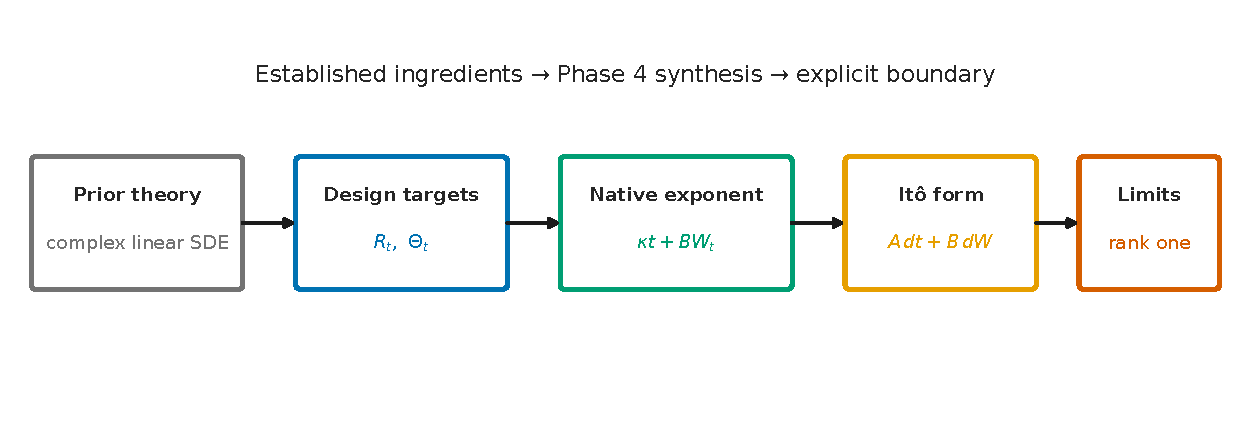
\includegraphics[width=1\linewidth,height=\textheight,keepaspectratio,alt={Flow diagram separating established complex linear SDE theory from the Phase 4 parameter synthesis and its rank-one limitation.}]{figures/vector/f01_research_claim_map.pdf}

}

\caption{\label{fig-research-claim-map}Flow diagram separating
established complex linear SDE theory from the Phase 4 parameter
synthesis and its rank-one limitation.}

\end{figure}%

Figure~\ref{fig-research-claim-map} states the claim hierarchy used
throughout this paper. Itô's formula, scalar complex linear SDEs,
complex GBM, and stochastic exponentials are established (Itô 1951;
Doléans-Dade 1970; Higham 2001; Buckwar et al. 2006). Our contribution
is a transparent parameter synthesis, geometric interpretation, exact
one-step formula, and reproducible boundary analysis. We do not claim to
have invented complex GBM.

A second distinction is equally important. The informal notation
\((dW_t)^2=dt\) summarizes quadratic variation; \(i^2=-1\) is an
algebraic identity. They are not the same statement. Complex
multiplication organizes scale and rotation, while quadratic variation
supplies the second-order term in Itô's formula. The connection is
through calculus, not through an identification of the two rules.

\section{Literature and positioning}\label{sec-literature}

Itô's original change-of-variables formula establishes the second-order
correction that distinguishes stochastic from ordinary differential
calculus (Itô 1951). Doléans-Dade's work places multiplicative solutions
in the semimartingale exponential framework (Doléans-Dade 1970). Modern
treatments make the relation between stochastic exponentials and
logarithms explicit (Larsson and Ruf 2019), while semimartingale
representation and multiplicative compensation frameworks include
complex-valued processes (Černý and Ruf 2022, 2023).

For the constant-coefficient scalar linear equation,

\[
dX_t=\lambda X_t\,dt+\eta X_t\,dW_t,
\]

Higham uses the exact exponential solution as a central analytical and
computational benchmark (Higham 2001). Buckwar, Horváth-Bokor, and
Winkler allow the state and coefficients to be complex, keep \(W\) real,
and explicitly call the exact solution ``complex geometric Brownian
motion'' in the full text (p.~262) (Buckwar et al. 2006). Perret
independently uses the same terminology for the scalar complex linear
SDE with multiplicative real noise (Perret 2010). Complex scalar linear
test equations also appear in numerical stability analysis (Abdulle et
al. 2013), and direction-and-norm decompositions provide related
geometric context for multiplicative-noise schemes (Mora et al. 2015).

The present process is therefore an established complex linear SDE under
a particular parameterization. What the parameterization accomplishes is
to preserve the ordinary GBM meanings of \((\mu,\sigma)\) in the modulus
while assigning independent modeling meanings to \((\omega,\beta)\) in
the phase. It also reveals the correction needed when translating those
log-polar targets to the Itô SDE coefficients.

Classical planar Brownian motion is a different object. Its two
Cartesian Brownian coordinates yield two noise directions, and its
winding theory has distinct asymptotic laws (Spitzer 1958; Pitman and
Yor 1986). Those references are used here only to mark the distinction.
A single real \(W\), even when multiplied by a complex number, still
supplies one instantaneous random direction.

The full source and claim audit is preserved in
\texttt{RESEARCH\_NOTES.md}. The audit deliberately excludes claims that
the complex GBM family, stochastic exponential, or exact scalar linear
solution is new.

\section{Preliminaries and notation}\label{sec-preliminaries}

Let \((\Omega,\mathcal F,(\mathcal F_t)_{t\ge0},\mathbb P)\) satisfy the
usual conditions, and let \(W=(W_t)_{t\ge0}\) be a standard
\textbf{real} Brownian motion. Brownian quadratic variation is

\begin{equation}\protect\phantomsection\label{eq-brownian-bracket}{
[W,W]_t=t,
}\end{equation}

or differentially \(d[W,W]_t=dt\). For a partition
\(\pi=\{0=t_0<\cdots<t_n=t\}\), this means

\[
\sum_{k=0}^{n-1}(W_{t_{k+1}}-W_{t_k})^2
\longrightarrow t
\]

in probability as the mesh tends to zero; it is not an ordinary
finite-increment identity (Mörters and Peres 2010).

We take

\[
\mu,\sigma,\omega,\beta\in\mathbb R,\qquad
\mathcal Z_0\in\mathbb C\setminus\{0\},
\]

and choose an initial phase lift \(\Theta_0\) satisfying
\(\mathcal Z_0=R_0e^{i\Theta_0}\), where \(R_0=|\mathcal Z_0|>0\).
Define

\begin{equation}\protect\phantomsection\label{eq-kappa-B}{
\kappa
=
\left(\mu-\frac12\sigma^2\right)+i\omega,\qquad
B=\sigma+i\beta.
}\end{equation}

We use two complex brackets:

\[
[Z,Z]_t
\quad\text{and}\quad
[Z,\overline Z]_t.
\]

The first is bilinear and can be complex. The second is Hermitian and
nonnegative. Conflating them replaces \(B^2\) by \(|B|^2\) and changes
the model.

``Native complex'' is operational language in this paper. It means that
the defining formula uses \(\mathcal Z_0\), \(W_t\), and complex
coefficients directly. It does not claim invariance under arbitrary
coordinate changes. Cartesian components may be plotted later, but they
are consequences rather than primitives.

\section{Problem formulation}\label{sec-problem}

We seek a nonzero complex process satisfying five requirements:

\begin{enumerate}
\def\labelenumi{\arabic{enumi}.}
\tightlist
\item
  its definition contains no separately evolved \(X_t\) and \(Y_t\);
\item
  its modulus is a real GBM with parameters \((\mu,\sigma)\);
\item
  its continuous phase has drift \(\omega\) and Brownian coefficient
  \(\beta\);
\item
  one finite Brownian increment produces an exact multiplicative step;
  and
\item
  the number of stochastic drivers remains explicit.
\end{enumerate}

A Cartesian-first definition \(Z_t=X_t+iY_t\) does not answer the first
requirement. A post-processing map \(Z_t=f(S_t)\) of a pre-existing
scalar state also leaves the original coordinate system in the
definition. Instead, we specify the complex log increment itself:

\[
d\Lambda_t=\kappa\,dt+B\,dW_t,\qquad \Lambda_0=0,
\]

and exponentiate:

\[
\mathcal Z_t=\mathcal Z_0e^{\Lambda_t}.
\]

\begin{figure}[tbp]

\centering{

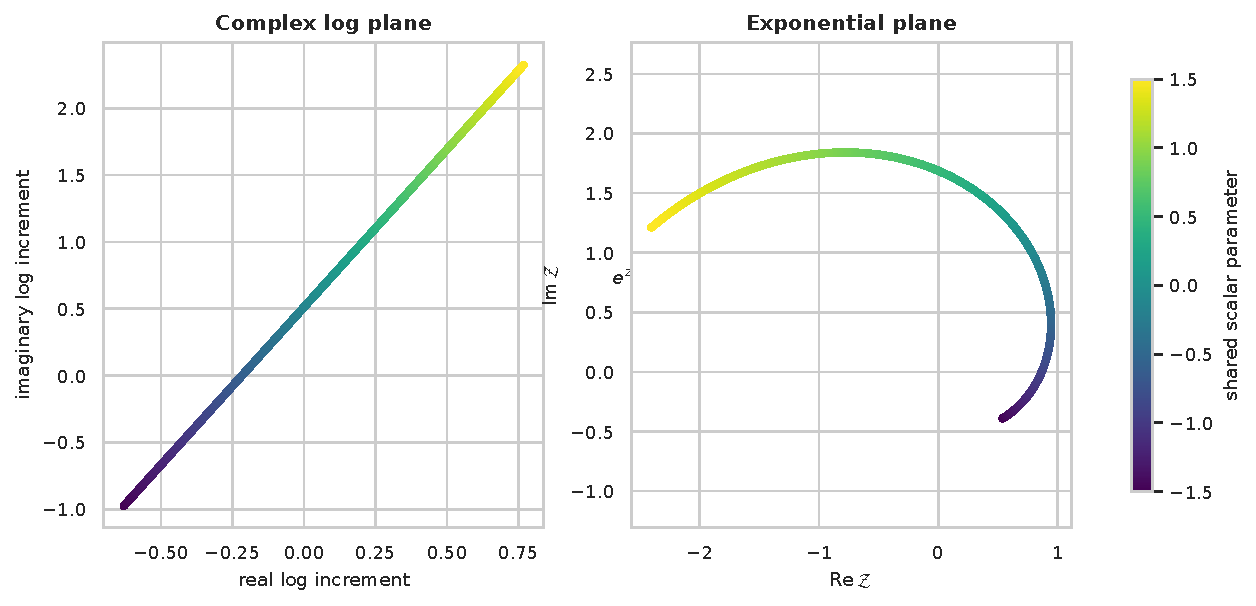
\includegraphics[width=1\linewidth,height=\textheight,keepaspectratio,alt={A colored line in the complex log plane maps through the exponential to a rotating curve with changing radius in the complex plane.}]{figures/vector/f02_log_to_exponential_plane.pdf}

}

\caption{\label{fig-log-exponential}A colored line in the complex log
plane maps through the exponential to a rotating curve with changing
radius in the complex plane.}

\end{figure}%

The two panels of Figure~\ref{fig-log-exponential} show the organizing
geometry. A single scalar Gaussian coordinate moves along an affine
direction in the complex log plane. Exponentiation converts its real
component to log scale and its imaginary component to phase.

\section{Native complex exponential
construction}\label{sec-construction}

\subsection{Direct definition}\label{direct-definition}

For \(t\ge0\), define the process by Eq.~\ref{eq-central-process},
equivalently

\begin{equation}\protect\phantomsection\label{eq-native-short}{
\mathcal Z_t=\mathcal Z_0e^{\kappa t+BW_t}.
}\end{equation}

The sample paths are continuous and adapted. Since the complex
exponential never vanishes,

\[
\mathcal Z_0\ne0
\quad\Longrightarrow\quad
\mathcal Z_t\ne0
\quad\text{for every finite }t
\]

pathwise. This avoids the zero-crossing and local-time complications
that arise when a signed real process is encoded literally as a polar
radius.

\subsection{Four-parameter separation}\label{four-parameter-separation}

Taking the real and imaginary parts of the exponent yields

\[
\operatorname{Re}(\kappa t+BW_t)
=
\left(\mu-\frac12\sigma^2\right)t+\sigma W_t,
\]

\[
\operatorname{Im}(\kappa t+BW_t)
=
\omega t+\beta W_t.
\]

The same \(W_t\) appears in both. The parameters are freely specifiable,
but the realized log-radius and phase noise are perfectly coupled
whenever \(\sigma\beta\ne0\).

\section{Exact modulus and continuous phase}\label{sec-modulus-phase}

\subsection{Modulus}\label{modulus}

Using \(|e^z|=e^{\operatorname{Re}z}\),

\begin{equation}\protect\phantomsection\label{eq-radius}{
\boxed{
R_t:=|\mathcal Z_t|
=
R_0\exp\!\left[
\left(\mu-\frac12\sigma^2\right)t+\sigma W_t
\right].
}
}\end{equation}

Applying real Itô calculus gives

\begin{equation}\protect\phantomsection\label{eq-radius-sde}{
\boxed{
\frac{dR_t}{R_t}=\mu\,dt+\sigma\,dW_t.
}
}\end{equation}

Thus the rotational parameters \(\omega\) and \(\beta\) do not alter the
modulus law. The equality is pathwise, not merely distributional.

\subsection{Phase lift}\label{phase-lift}

Define

\begin{equation}\protect\phantomsection\label{eq-phase}{
\boxed{
\Theta_t=\Theta_0+\omega t+\beta W_t.
}
}\end{equation}

Then

\[
\mathcal Z_t=R_te^{i\Theta_t}.
\]

\(\Theta\) is a continuous unwrapped phase. The principal argument
\(\operatorname{Arg}\mathcal Z_t\in(-\pi,\pi]\) may jump by \(2\pi\) at
its branch cut even though \(\mathcal Z\) and \(\Theta\) are continuous.
We therefore never silently identify the continuous lift with the
principal branch.

\begin{figure}[tbp]

\centering{

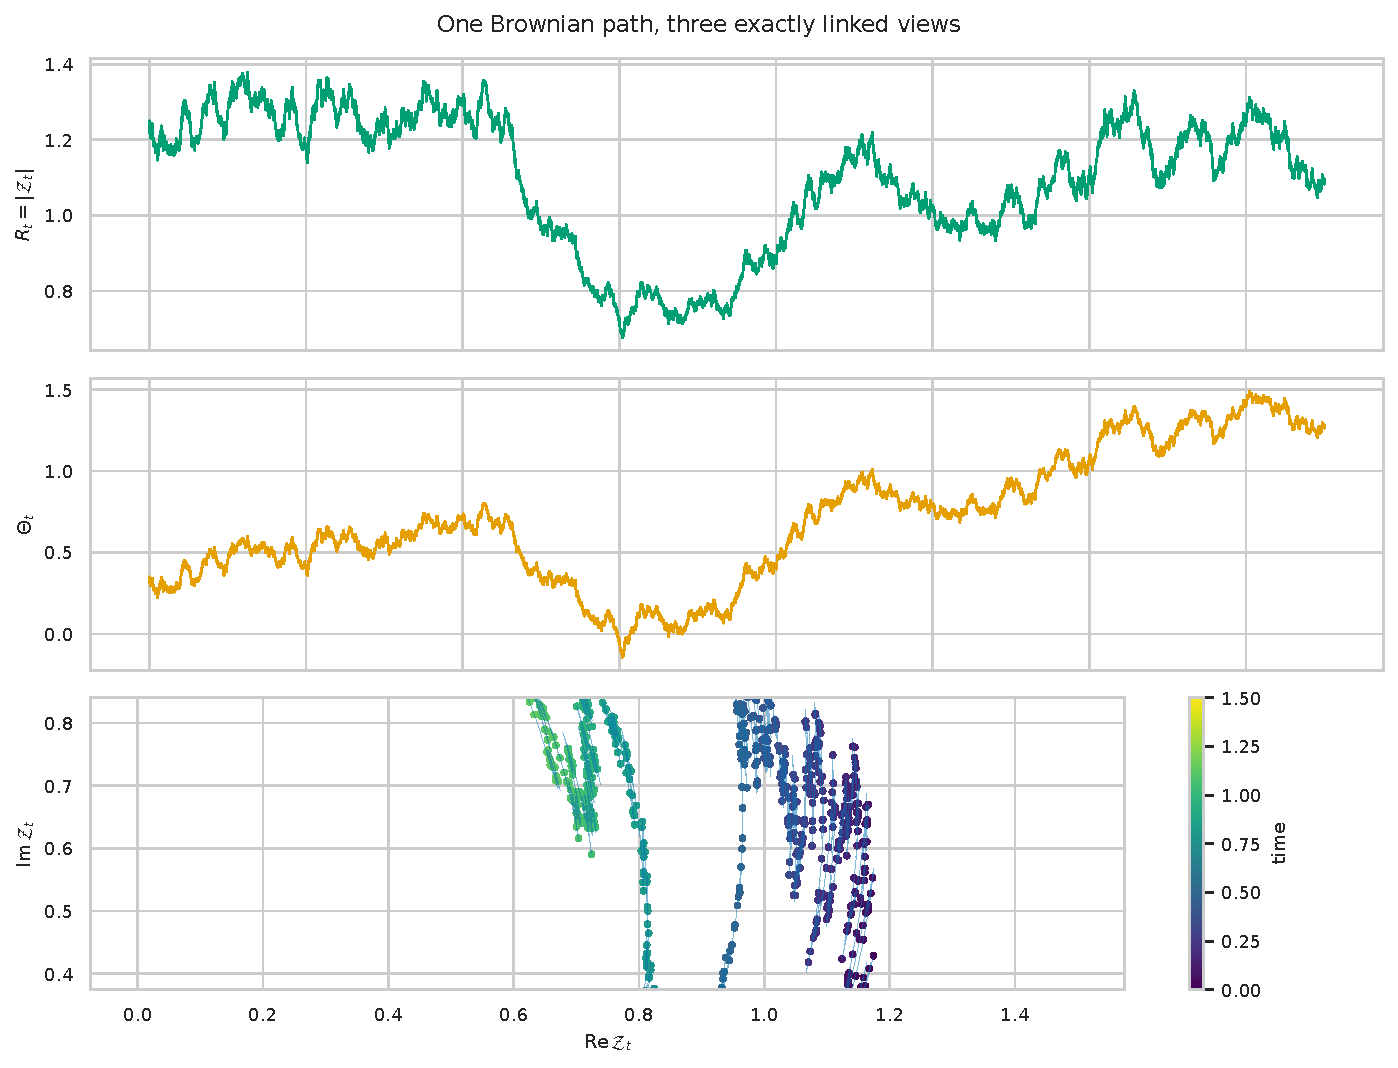
\includegraphics[width=0.95\linewidth,height=\textheight,keepaspectratio,alt={Three panels show the exact GBM modulus, continuous unwrapped phase, and resulting complex trajectory generated by one Brownian path.}]{figures/vector/f03_linked_modulus_phase_path.pdf}

}

\caption{\label{fig-linked-path}Three panels show the exact GBM modulus,
continuous unwrapped phase, and resulting complex trajectory generated
by one Brownian path.}

\end{figure}%

Figure~\ref{fig-linked-path} shows three views of one Brownian
realization. Neither the radius nor the phase is fixed, yet no second
random input has been introduced.

\begin{figure}[tbp]

\centering{


\includegraphics[width=0.85\linewidth,height=\textheight,keepaspectratio,alt={Three-dimensional curve showing real part, imaginary part, and time for one exact native complex geometric Brownian motion path.}]{figures/vector/f04_space_time_trajectory.pdf}

}

\caption{\label{fig-space-time}Three-dimensional curve showing real
part, imaginary part, and time for one exact native complex geometric
Brownian motion path.}

\end{figure}%

The space-time view in Figure~\ref{fig-space-time} prevents a common
visual misinterpretation: a path drawn in a plane is not necessarily
driven by two-dimensional Brownian noise.

\begin{figure}[tbp]

\centering{

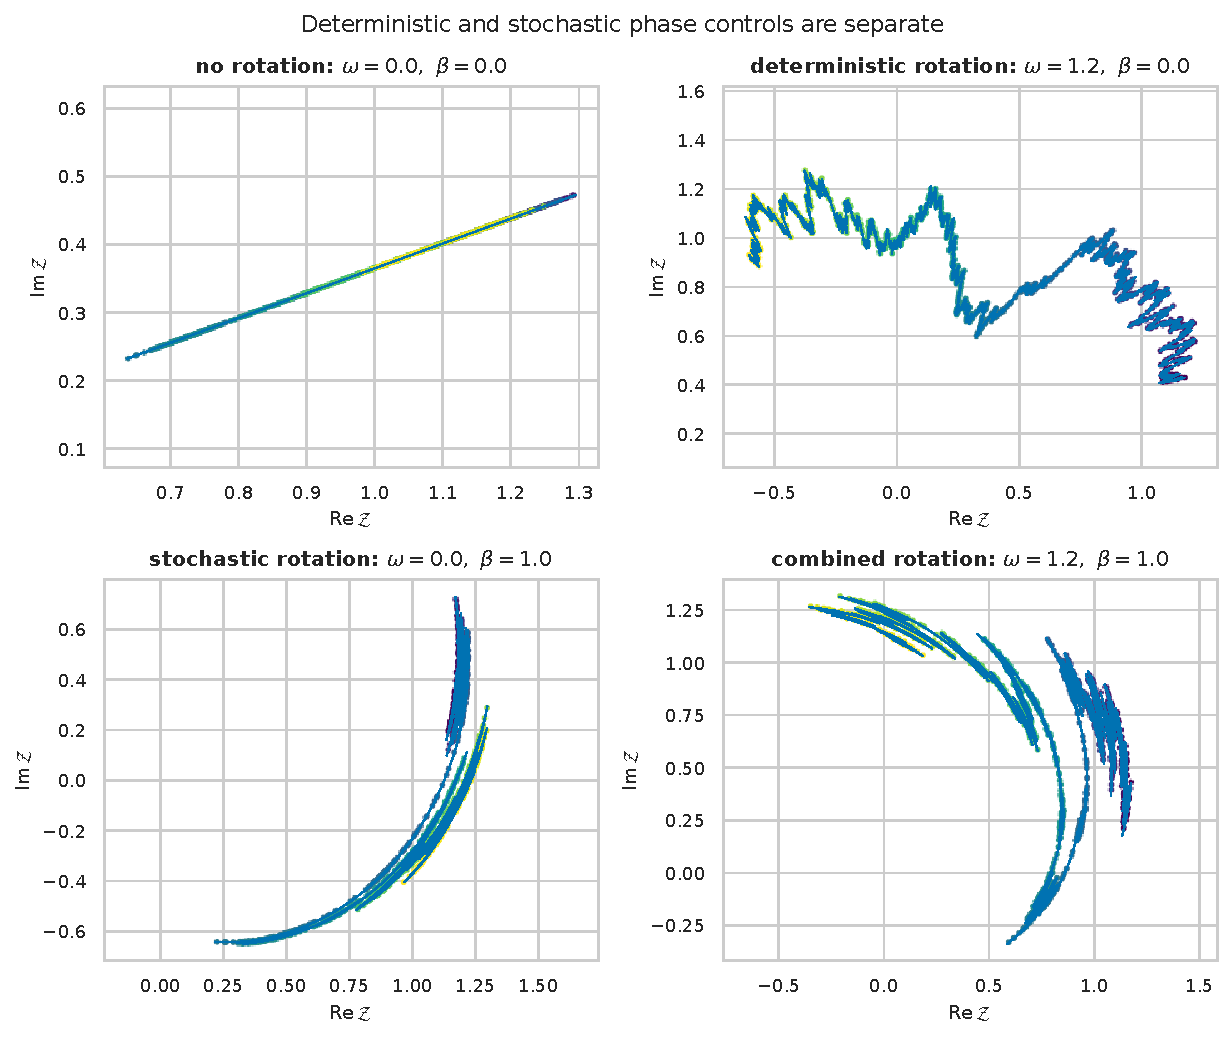
\includegraphics[width=0.88\linewidth,height=\textheight,keepaspectratio,alt={Four complex paths compare absent, deterministic, stochastic, and combined rotation while keeping the same radial GBM parameters and Brownian path.}]{figures/vector/f05_rotation_parameter_gallery.pdf}

}

\caption{\label{fig-rotation-gallery}Four complex paths compare absent,
deterministic, stochastic, and combined rotation while keeping the same
radial GBM parameters and Brownian path.}

\end{figure}%

Figure~\ref{fig-rotation-gallery} varies only \((\omega,\beta)\) while
holding the radial parameters and Brownian path fixed. Deterministic
rotation changes the phase trend; stochastic rotation changes the
phase's quadratic variation.

\section{Complex Itô dynamics}\label{sec-ito-dynamics}

Let \(F(z)=e^z\) and \(\Lambda_t=\kappa t+BW_t\). The complex
exponential is entire, so applying Itô's formula componentwise gives

\[
d(e^{\Lambda_t})
=
e^{\Lambda_t}d\Lambda_t
+\frac12e^{\Lambda_t}d[\Lambda,\Lambda]_t.
\]

Because the bracket is bilinear,

\[
d[\Lambda,\Lambda]_t=B^2dt.
\]

Therefore

\begin{equation}\protect\phantomsection\label{eq-ito-compact}{
\frac{d\mathcal Z_t}{\mathcal Z_t}
=
\left(\kappa+\frac12B^2\right)dt+B\,dW_t.
}\end{equation}

Set \(A=\kappa+B^2/2\). Expanding the square,

\[
B^2=(\sigma+i\beta)^2
=\sigma^2-\beta^2+2i\sigma\beta,
\]

so

\begin{equation}\protect\phantomsection\label{eq-drift-A}{
\boxed{
A
=
\mu-\frac12\beta^2+i(\omega+\sigma\beta).
}
}\end{equation}

The native complex Itô SDE is

\begin{equation}\protect\phantomsection\label{eq-final-sde}{
\boxed{
\frac{d\mathcal Z_t}{\mathcal Z_t}
=
\left[
\mu-\frac12\beta^2+i(\omega+\sigma\beta)
\right]dt
+(\sigma+i\beta)dW_t.
}
}\end{equation}

Two corrections must be retained:

\begin{itemize}
\tightlist
\item
  \(-\beta^2/2\) compensates the radial effect of stochastic rotation;
  and
\item
  \(+\sigma\beta\) is the imaginary cross drift caused by a shared
  driver.
\end{itemize}

These terms are forced by the target modulus and phase. Conversely,
starting from \(B=\sigma+i\beta\) and demanding \(A-B^2/2=\kappa\)
determines \(A\) uniquely.

\subsection{Pure stochastic rotation stress
test}\label{pure-stochastic-rotation-stress-test}

Take \(\mu=\sigma=0\). Then

\[
\mathcal Z_t=\mathcal Z_0e^{i\omega t+i\beta W_t}
\]

has constant modulus. Its SDE nevertheless contains a real drift:

\[
\frac{d\mathcal Z_t}{\mathcal Z_t}
=
\left(-\frac12\beta^2+i\omega\right)dt+i\beta\,dW_t.
\]

If the term \(-\beta^2/2\) is omitted from the SDE drift, the
corresponding exact solution acquires the spurious radial factor
\(e^{\beta^2t/2}\).

\begin{figure}[tbp]

\centering{

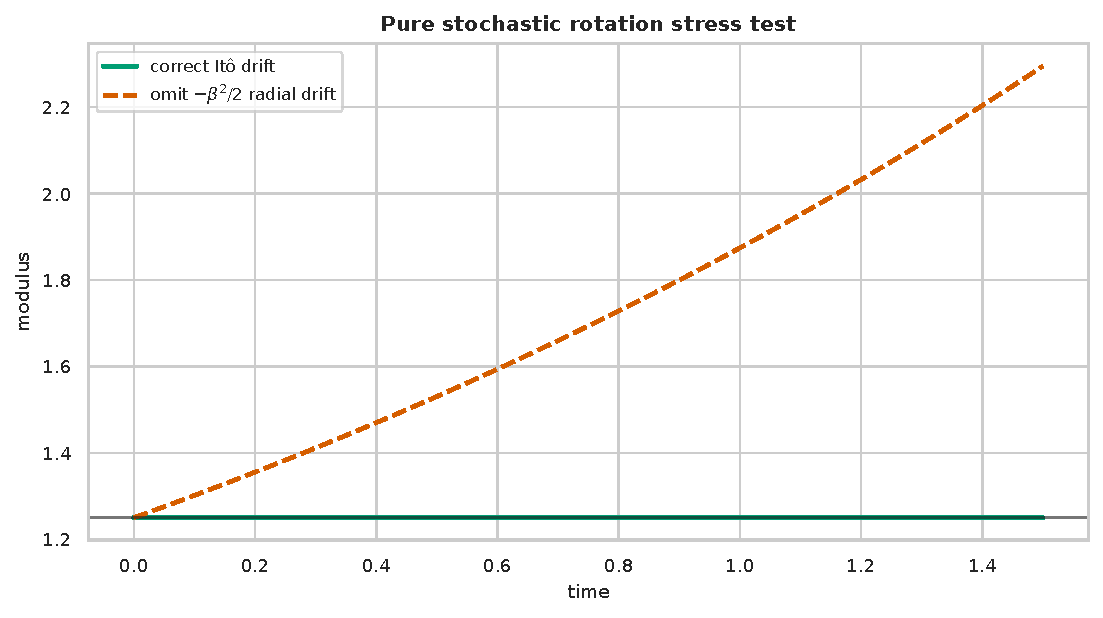
\includegraphics[width=0.82\linewidth,height=\textheight,keepaspectratio,alt={The correctly compensated pure stochastic rotation keeps constant modulus, while omitting the negative half beta-squared Itô drift creates spurious radial growth.}]{figures/vector/f06_constant_modulus_correction.pdf}

}

\caption{\label{fig-constant-modulus}The correctly compensated pure
stochastic rotation keeps constant modulus, while omitting the negative
half beta-squared Itô drift creates spurious radial growth.}

\end{figure}%

Figure~\ref{fig-constant-modulus} is a direct diagnostic of the Itô
correction. Rotation generated by Brownian phase is not ordinary
differentiable rotation.

\section{Stochastic exponential and
logarithm}\label{sec-stochastic-exponential}

Let

\[
Y_t=At+BW_t.
\]

For a continuous semimartingale, the Doléans exponential is

\[
\mathcal E(Y)_t
=
\exp\!\left(Y_t-Y_0-\frac12[Y,Y]_t\right)
\]

(Doléans-Dade 1970; Larsson and Ruf 2019). Since \([Y,Y]_t=B^2t\),

\[
\mathcal E(Y)_t
=
\exp\!\left[
\left(A-\frac12B^2\right)t+BW_t
\right]
=e^{\kappa t+BW_t}.
\]

Hence

\begin{equation}\protect\phantomsection\label{eq-doleans-form}{
\boxed{
\mathcal Z_t=\mathcal Z_0\mathcal E(Y)_t.
}
}\end{equation}

This reconciles the ordinary and stochastic exponentials. The continuous
ordinary log lift and the stochastic logarithm are related but not
identical:

\[
\log_{\mathrm{cont}}\frac{\mathcal Z_t}{\mathcal Z_0}
=\kappa t+BW_t,
\]

whereas

\[
\mathcal L\!\left(\frac{\mathcal Z}{\mathcal Z_0}\right)_t
:=
\int_0^t\frac{d\mathcal Z_s}{\mathcal Z_s}
=At+BW_t.
\]

Their difference is the half-bracket correction \(B^2t/2\). This is the
complex analogue of the familiar distinction between the log return and
the arithmetic drift of real GBM.

\section{Exact transition and random-walk
formula}\label{sec-exact-transition}

For a grid \(t_n\) with step \(h=t_{n+1}-t_n\), define
\(\Delta W_n=W_{t_{n+1}}-W_{t_n}\sim N(0,h)\). Independent Brownian
increments give

\begin{equation}\protect\phantomsection\label{eq-exact-step}{
\boxed{
\mathcal Z_{n+1}
=
\mathcal Z_n
\exp\!\left(
\left[\left(\mu-\frac12\sigma^2\right)+i\omega\right]h
+(\sigma+i\beta)\Delta W_n
\right).
}
}\end{equation}

This is an exact random walk on the multiplicative group
\(\mathbb C\setminus\{0\}\). One complex log increment combines:

\[
\Delta\log R_n
=
\left(\mu-\frac12\sigma^2\right)h+\sigma\Delta W_n,
\]

\[
\Delta\Theta_n
=
\omega h+\beta\Delta W_n.
\]

\begin{figure}[tbp]

\centering{

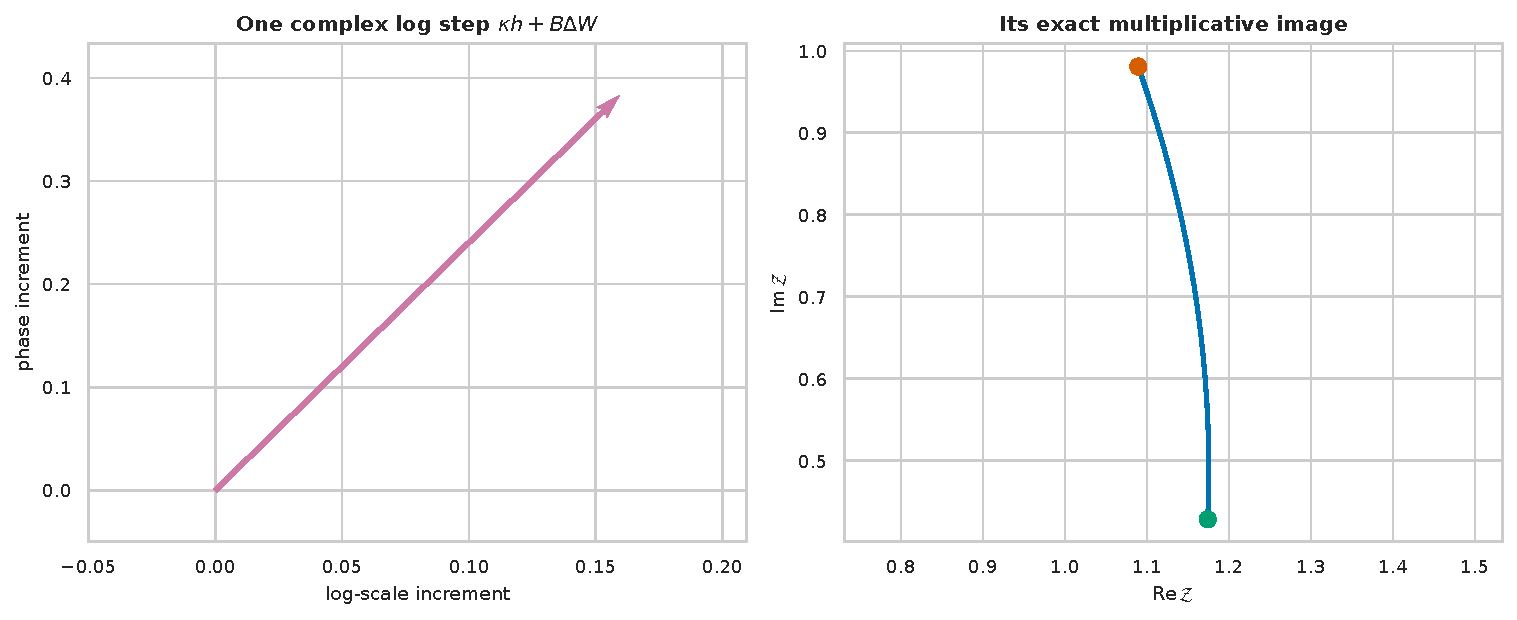
\includegraphics[width=0.95\linewidth,height=\textheight,keepaspectratio,alt={A complex log increment is shown as one vector whose exponential maps an initial state to the next state along a scale-and-rotation arc.}]{figures/vector/f07_exact_step_geometry.pdf}

}

\caption{\label{fig-exact-step}A complex log increment is shown as one
vector whose exponential maps an initial state to the next state along a
scale-and-rotation arc.}

\end{figure}%

Figure~\ref{fig-exact-step} visualizes the step in the log plane and its
multiplicative image. Unlike Euler--Maruyama, Eq.~\ref{eq-exact-step}
has no time-discretization error for the constant-coefficient model.

\section{Transition laws and moments}\label{sec-laws-moments}

\subsection{Singular log-polar Gaussian
law}\label{singular-log-polar-gaussian-law}

At time \(t\),

\begin{equation}\protect\phantomsection\label{eq-log-polar-law}{
\begin{pmatrix}
\log(R_t/R_0)\\
\Theta_t-\Theta_0
\end{pmatrix}
\sim
\mathcal N\!\left(
\begin{pmatrix}
(\mu-\sigma^2/2)t\\
\omega t
\end{pmatrix},
t
\begin{pmatrix}
\sigma^2&\sigma\beta\\
\sigma\beta&\beta^2
\end{pmatrix}
\right).
}\end{equation}

The covariance determinant is zero:

\[
\sigma^2\beta^2-(\sigma\beta)^2=0.
\]

If \(\sigma\ne0\), the support line is

\begin{equation}\protect\phantomsection\label{eq-support-line}{
\Theta_t-\Theta_0-\omega t
=
\frac{\beta}{\sigma}
\left[
\log(R_t/R_0)-\left(\mu-\frac12\sigma^2\right)t
\right].
}\end{equation}

\begin{figure}[tbp]

\centering{

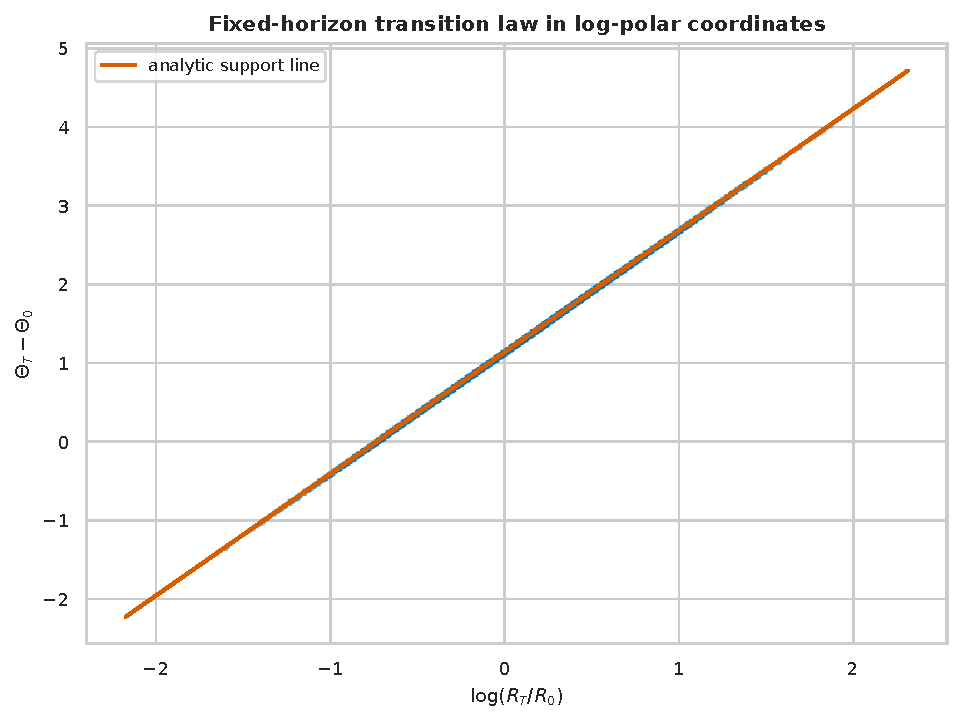
\includegraphics[width=0.8\linewidth,height=\textheight,keepaspectratio,alt={A fixed-horizon log-radius and phase sample lies on the analytic rank-one Gaussian support line in log-polar coordinates.}]{figures/vector/f08_log_polar_transition.pdf}

}

\caption{\label{fig-log-polar-transition}A fixed-horizon log-radius and
phase sample lies on the analytic rank-one Gaussian support line in
log-polar coordinates.}

\end{figure}%

The simulated transition sample in Figure~\ref{fig-log-polar-transition}
lies on Eq.~\ref{eq-support-line} up to floating-point plotting
precision.

At fixed \(t\), the complex support is parameterized by one real
coordinate:

\[
\left\{
\mathcal Z_0e^{\kappa t+Bw}:w\in\mathbb R
\right\}.
\]

For \(\sigma\beta\ne0\), this is a logarithmic spiral. Degenerate cases
become a ray (\(\beta=0\)) or a circle traced through wrapped phase
(\(\sigma=0,\beta\ne0\)).

\begin{figure}[tbp]

\centering{

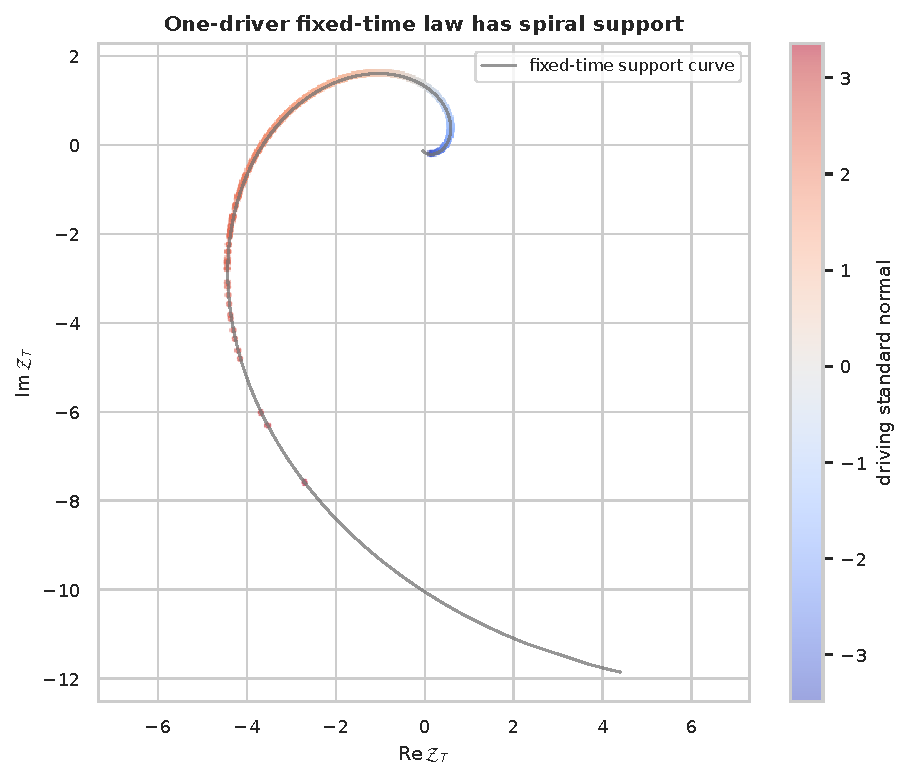
\includegraphics[width=0.8\linewidth,height=\textheight,keepaspectratio,alt={Terminal complex samples from one real Brownian driver lie on a one-dimensional logarithmic spiral rather than filling a two-dimensional region.}]{figures/vector/f09_fixed_time_spiral_support.pdf}

}

\caption{\label{fig-fixed-support}Terminal complex samples from one real
Brownian driver lie on a one-dimensional logarithmic spiral rather than
filling a two-dimensional region.}

\end{figure}%

Figure~\ref{fig-fixed-support} shows why a complex-valued law need not
have a two-dimensional density with respect to planar area.

\subsection{Radial moments}\label{radial-moments}

For real \(p\) for which the expression is considered,

\begin{equation}\protect\phantomsection\label{eq-radial-moment}{
\boxed{
\mathbb E[R_t^p]
=
R_0^p
\exp\!\left[
\left(
p\mu+\frac12p(p-1)\sigma^2
\right)t
\right].
}
}\end{equation}

All real powers have finite moments at finite \(t\) because \(R_t\) is
lognormal.

\subsection{Complex integer moments}\label{complex-integer-moments}

For integer \(n\),

\begin{equation}\protect\phantomsection\label{eq-complex-moment}{
\boxed{
\mathbb E[\mathcal Z_t^n]
=
\mathcal Z_0^n
\exp\!\left[
\left(n\kappa+\frac12n^2B^2\right)t
\right].
}
}\end{equation}

The complex square \(B^2\) determines both amplification or damping and
rotation of the moment.

\subsection{Mixed log-polar moments}\label{mixed-log-polar-moments}

For real \(p,q\),

\begin{equation}\protect\phantomsection\label{eq-mixed-moment}{
\boxed{
\mathbb E\!\left[
R_t^p e^{iq(\Theta_t-\Theta_0)}
\right]
=
R_0^p
\exp\!\left[
p\left(\mu-\frac12\sigma^2\right)t
+iq\omega t
+\frac12(p\sigma+iq\beta)^2t
\right].
}
}\end{equation}

This formula exposes the shared-driver coupling through the cross term
in \((p\sigma+iq\beta)^2\).

\begin{figure}[tbp]

\centering{

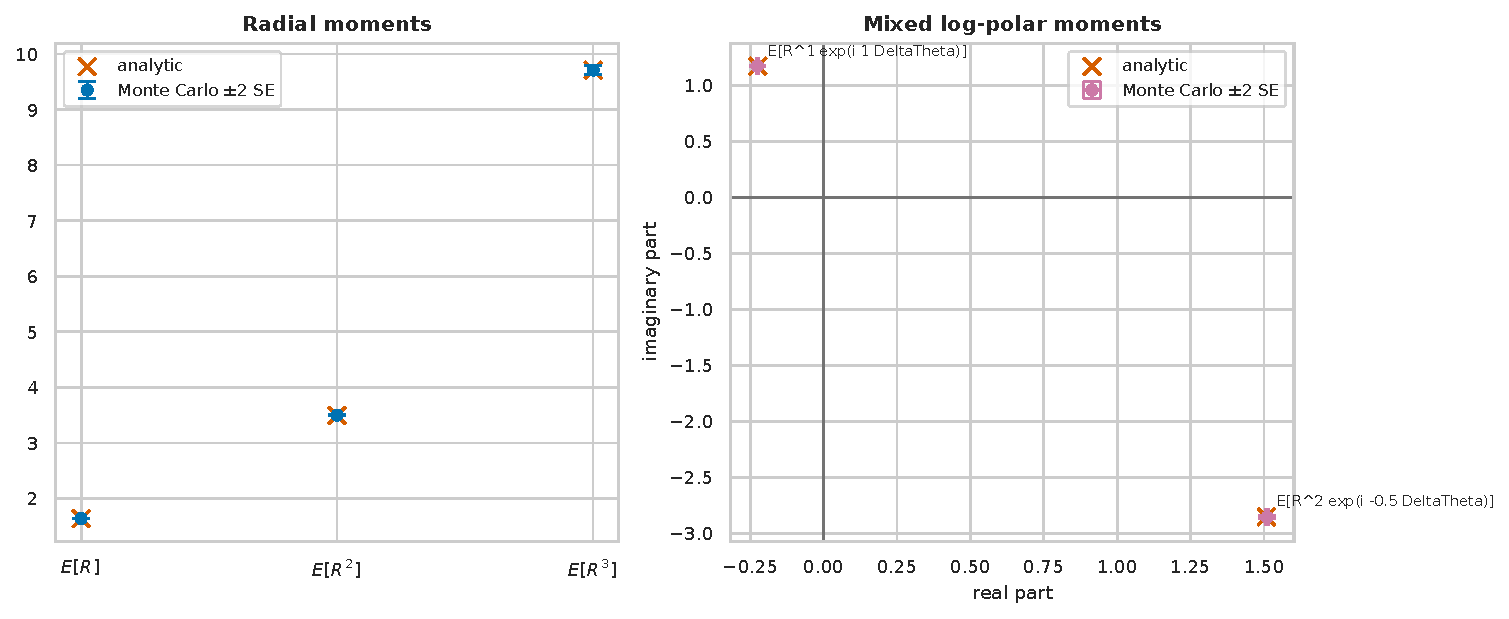
\includegraphics[width=0.95\linewidth,height=\textheight,keepaspectratio,alt={Analytic radial and mixed log-polar moments agree with seeded Monte Carlo estimates and their componentwise two-standard-error bars.}]{figures/vector/f13_moment_validation.pdf}

}

\caption{\label{fig-moment-validation}Analytic radial and mixed
log-polar moments agree with seeded Monte Carlo estimates and their
componentwise two-standard-error bars.}

\end{figure}%

Figure~\ref{fig-moment-validation} compares these formulas with
independent terminal samples. The estimates are a numerical check;
Gaussian evaluation proves the identities.

\begin{figure}[tbp]

\centering{

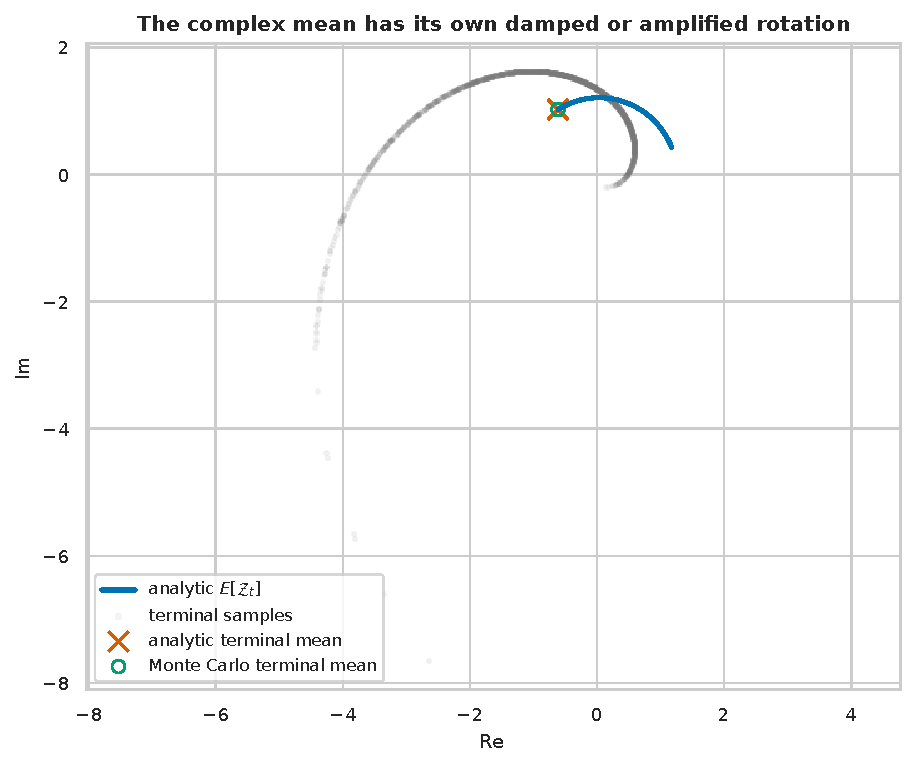
\includegraphics[width=0.76\linewidth,height=\textheight,keepaspectratio,alt={The analytic complex mean traces a deterministic curve through time and ends at the same point as the seeded Monte Carlo terminal mean.}]{figures/vector/f14_complex_mean_geometry.pdf}

}

\caption{\label{fig-complex-mean}The analytic complex mean traces a
deterministic curve through time and ends at the same point as the
seeded Monte Carlo terminal mean.}

\end{figure}%

The first moment in Figure~\ref{fig-complex-mean} need not rotate at the
same rate as an individual path because the term \(B^2/2\) changes both
its real and imaginary exponents.

\section{Geometry and noise dimension}\label{sec-geometry}

\subsection{Local Cartesian diffusion}\label{local-cartesian-diffusion}

Write \(\mathcal Z_t=X_t+iY_t\). This is a derived decomposition, not
the definition. The complex diffusion coefficient at state \(z\) is
\(Bz\), so the real two-vector multiplying \(dW_t\) is

\[
g(z)
=
\begin{pmatrix}
\operatorname{Re}(Bz)\\
\operatorname{Im}(Bz)
\end{pmatrix}.
\]

The instantaneous Cartesian covariance is

\[
g(z)g(z)^\mathsf T\,dt.
\]

It is an outer product and therefore has rank at most one. Both radial
and tangential components may be nonzero, but a single scalar increment
chooses only one combined direction.

\begin{figure}[tbp]

\centering{

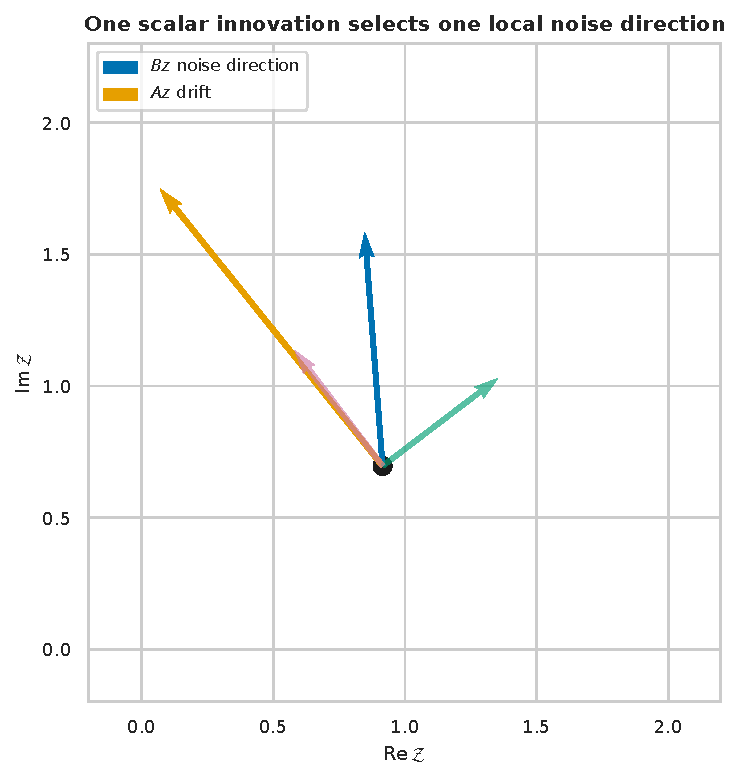
\includegraphics[width=0.72\linewidth,height=\textheight,keepaspectratio,alt={At one complex state, the diffusion vector has radial and tangential components but remains a single local noise direction driven by one scalar Brownian increment.}]{figures/vector/f10_local_noise_direction.pdf}

}

\caption{\label{fig-local-direction}At one complex state, the diffusion
vector has radial and tangential components but remains a single local
noise direction driven by one scalar Brownian increment.}

\end{figure}%

Figure~\ref{fig-local-direction} distinguishes ``two geometric
components'' from ``two independent stochastic directions.''

\subsection{Log-polar covariance rank}\label{log-polar-covariance-rank}

The martingale parts of log-radius and phase are

\[
dM_t^{(r)}=\sigma\,dW_t,\qquad
dM_t^{(\theta)}=\beta\,dW_t.
\]

Their covariance rate is

\begin{equation}\protect\phantomsection\label{eq-one-covariance}{
\boxed{
\Sigma_1
=
\begin{pmatrix}
\sigma^2&\sigma\beta\\
\sigma\beta&\beta^2
\end{pmatrix}
=
\begin{pmatrix}\sigma\\\beta\end{pmatrix}
\begin{pmatrix}\sigma&\beta\end{pmatrix}.
}
}\end{equation}

The nonzero eigenvalue is \(\sigma^2+\beta^2\); the other is zero. This
rank is invariant under any nonsingular deterministic change of the two
output coordinates. Coordinate notation cannot increase the input noise
dimension.

\begin{figure}[tbp]

\centering{

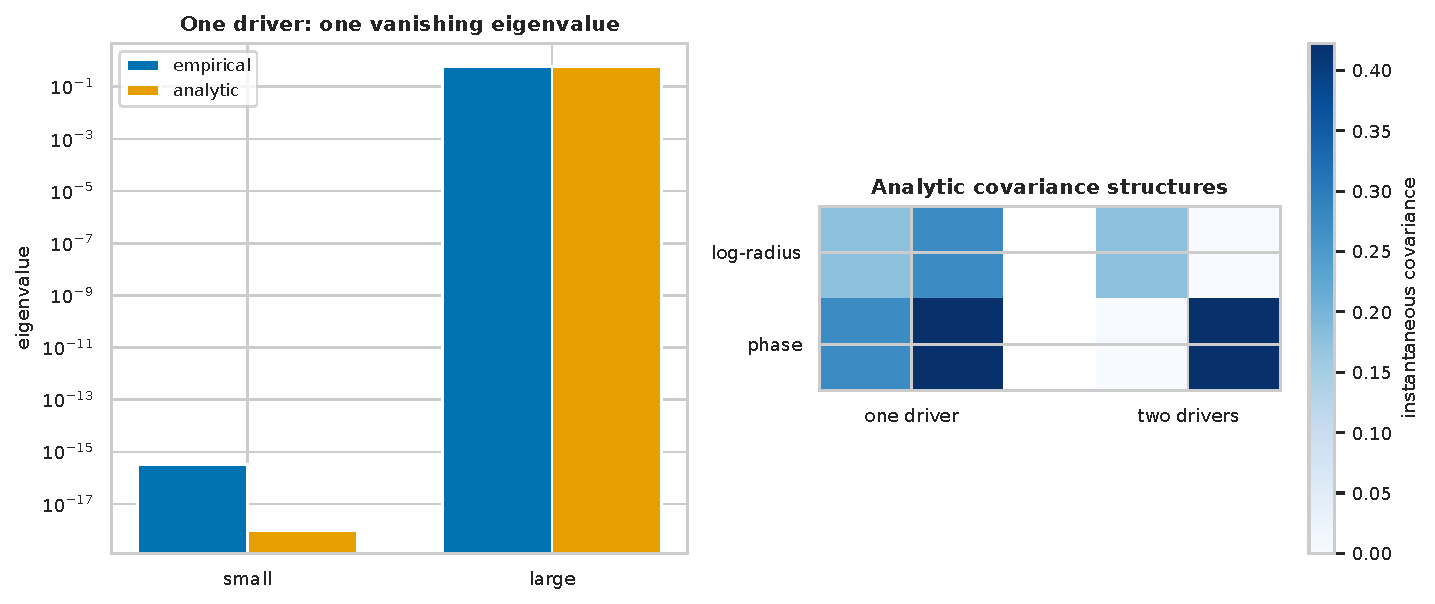
\includegraphics[width=0.95\linewidth,height=\textheight,keepaspectratio,alt={The one-driver covariance has one numerically vanishing eigenvalue, while a companion heatmap contrasts its outer-product structure with the two-driver diagonal covariance.}]{figures/vector/f11_covariance_eigenspectrum.pdf}

}

\caption{\label{fig-covariance-spectrum}The one-driver covariance has
one numerically vanishing eigenvalue, while a companion heatmap
contrasts its outer-product structure with the two-driver diagonal
covariance.}

\end{figure}%

The eigenvalue ratio reported by the notebook for
Figure~\ref{fig-covariance-spectrum} is \(5.54\times10^{-16}\),
numerical rank one.

\begin{figure}[tbp]

\centering{

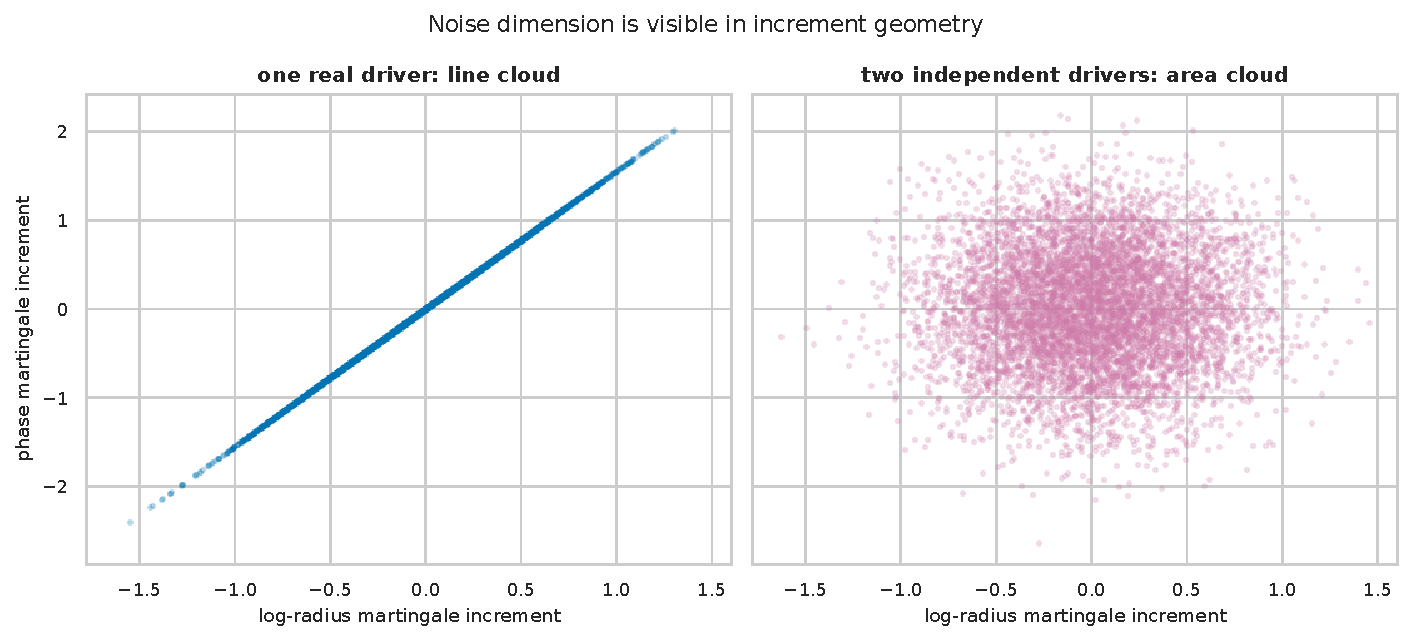
\includegraphics[width=0.92\linewidth,height=\textheight,keepaspectratio,alt={One-driver log-polar increments form a line, whereas independent radial and angular Brownian increments fill a two-dimensional elliptical cloud.}]{figures/vector/f12_one_vs_two_driver_clouds.pdf}

}

\caption{\label{fig-driver-clouds}One-driver log-polar increments form a
line, whereas independent radial and angular Brownian increments fill a
two-dimensional elliptical cloud.}

\end{figure}%

The two clouds in Figure~\ref{fig-driver-clouds} provide the most direct
visual test of the driver-count claim.

\subsection{Bilinear and Hermitian
brackets}\label{bilinear-and-hermitian-brackets}

From the diffusion \(B\mathcal Z_t\,dW_t\),

\begin{equation}\protect\phantomsection\label{eq-bilinear-bracket}{
\boxed{
d[\mathcal Z,\mathcal Z]_t
=B^2\mathcal Z_t^2\,dt,
}
}\end{equation}

and

\begin{equation}\protect\phantomsection\label{eq-hermitian-bracket}{
\boxed{
d[\mathcal Z,\overline{\mathcal Z}]_t
=|B|^2|\mathcal Z_t|^2\,dt.
}
}\end{equation}

The first preserves complex orientation information; the second is a
nonnegative accumulated energy. They answer different questions.

\section{Phase 3 and two-driver boundaries}\label{sec-boundaries}

\subsection{Phase 3 constrained
subfamily}\label{phase-3-constrained-subfamily}

Phase 3 used

\[
\mathcal Z_t
=
\mathcal Z_0e^{(1+i\gamma)L_t},
\]

where the real GBM log return is

\[
L_t
=
\left(\mu-\frac12\sigma^2\right)t+\sigma W_t.
\]

Expanding and matching Eq.~\ref{eq-central-process} gives the necessary
and sufficient restrictions

\begin{equation}\protect\phantomsection\label{eq-phase3-restrictions}{
\boxed{
\beta=\gamma\sigma,\qquad
\omega=\gamma\left(\mu-\frac12\sigma^2\right).
}
}\end{equation}

Thus Phase 3 ties the angular drift and diffusion to one spiral
coefficient \(\gamma\). Phase 4 permits \(\omega\) and \(\beta\) to be
chosen independently while preserving the same radial GBM.

\begin{figure}[tbp]

\centering{

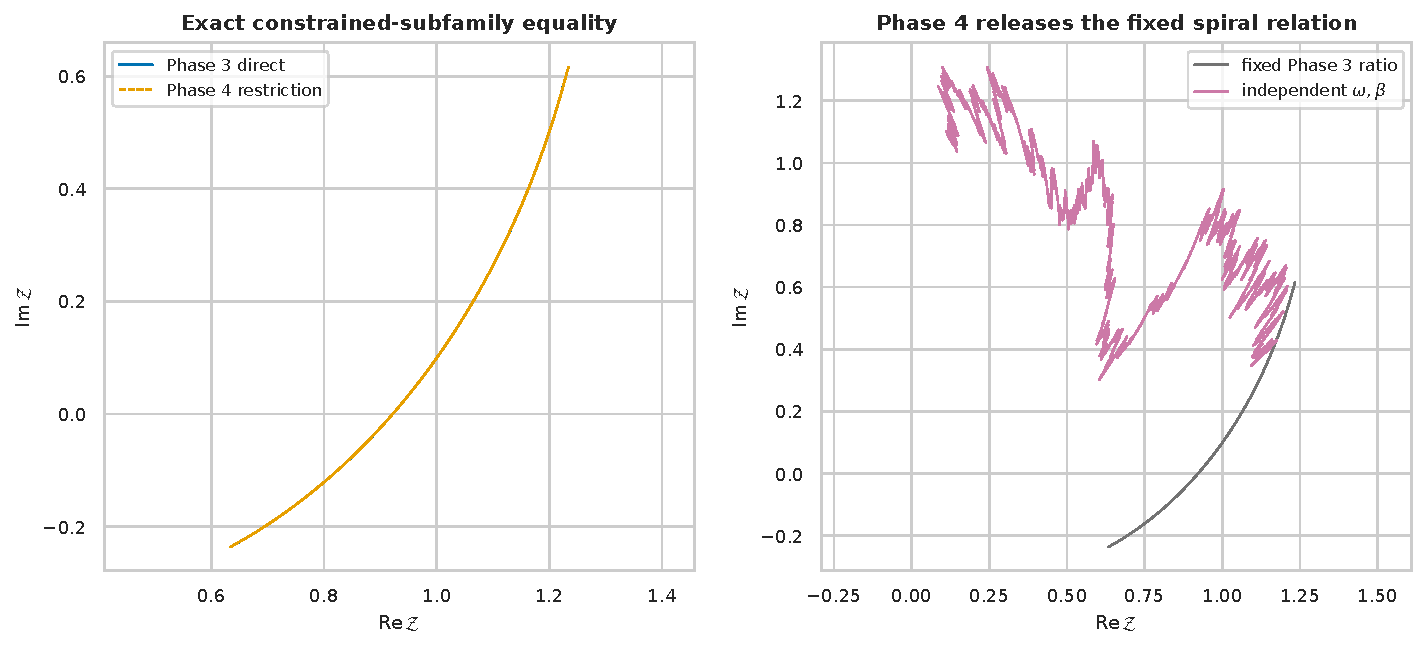
\includegraphics[width=0.92\linewidth,height=\textheight,keepaspectratio,alt={The Phase 3 logarithmic-spiral formula exactly overlaps the restricted Phase 4 process, while independently chosen phase parameters produce a different path.}]{figures/vector/f15_phase3_subfamily.pdf}

}

\caption{\label{fig-phase3-subfamily}The Phase 3 logarithmic-spiral
formula exactly overlaps the restricted Phase 4 process, while
independently chosen phase parameters produce a different path.}

\end{figure}%

The restricted paths in Figure~\ref{fig-phase3-subfamily} agree to
\(2.73\times10^{-16}\), the maximum pathwise discrepancy recorded in
\texttt{phase3\_equivalence.json}.

\subsection{Independent two-driver
comparator}\label{independent-two-driver-comparator}

Let \(W^{(r)}\) and \(W^{(\theta)}\) be independent real Brownian
motions and define

\begin{equation}\protect\phantomsection\label{eq-two-driver-process}{
\mathcal Z_t^{(2)}
=
\mathcal Z_0
\exp\!\left[
\kappa t+\sigma W_t^{(r)}+i\beta W_t^{(\theta)}
\right].
}\end{equation}

The modulus and phase targets remain

\[
\frac{dR_t^{(2)}}{R_t^{(2)}}=\mu\,dt+\sigma\,dW_t^{(r)},
\]

\[
d\Theta_t^{(2)}=\omega\,dt+\beta\,dW_t^{(\theta)},
\]

but their covariance rate becomes

\begin{equation}\protect\phantomsection\label{eq-two-covariance}{
\boxed{
\Sigma_2=
\begin{pmatrix}
\sigma^2&0\\
0&\beta^2
\end{pmatrix}.
}
}\end{equation}

It has rank two when \(\sigma\beta\ne0\). The Itô bracket of the complex
log increment is now

\[
\sigma^2dt+(i\beta)^2dt=(\sigma^2-\beta^2)dt,
\]

because the cross bracket of the independent drivers vanishes. Therefore

\begin{equation}\protect\phantomsection\label{eq-two-driver-sde}{
\boxed{
\frac{d\mathcal Z_t^{(2)}}{\mathcal Z_t^{(2)}}
=
\left(\mu-\frac12\beta^2+i\omega\right)dt
+\sigma\,dW_t^{(r)}
+i\beta\,dW_t^{(\theta)}.
}
}\end{equation}

Compared with Eq.~\ref{eq-final-sde}, the imaginary cross drift
\(\sigma\beta\) disappears. It is a signature of the one-driver
coupling, not a universal feature of complex notation.

\section{Numerical methods}\label{sec-methods}

\subsection{Reproducible design}\label{reproducible-design}

The executed discovery notebook imports the tested root
\texttt{phase4\_model.py}. It does not reimplement the model in an
isolated paper-only module. All random number generators use seeds
derived from 20260724. Figures are written as vector PDF files for the
printed paper and 300-dpi PNG companions for HTML. Every evidence table
is CSV or sorted JSON, and a manifest records all generated artifacts
and figure alt text.

The primary numerical parameters are

\[
(\mu,\sigma,\omega,\beta)=(0.18,0.42,0.90,0.65),
\]

with \(R_0=1.25\), \(\Theta_0=0.35\), and \(T=1.50\). These values are
illustrative and were fixed before reporting diagnostics.

The environment record is summarized below.

\begin{longtable}[]{@{}ll@{}}
\caption{Software versions from
\protect\texttt{tables/software\_versions.csv}.}\label{tbl-software}\tabularnewline
\toprule\noalign{}
Component & Version \\
\midrule\noalign{}
\endfirsthead
\toprule\noalign{}
Component & Version \\
\midrule\noalign{}
\endhead
\bottomrule\noalign{}
\endlastfoot
Python & 3.12.13 \\
NumPy & 2.5.1 \\
SciPy & 1.18.0 \\
pandas & 3.0.3 \\
Matplotlib & 3.11.1 \\
Seaborn & 0.13.2 \\
SymPy & 1.14.0 \\
nbformat & 5.10.4 \\
\end{longtable}

\subsection{Exact-identity checks}\label{exact-identity-checks}

One Brownian path with 8192 increments tests:

\begin{itemize}
\tightlist
\item
  \(A-B^2/2=\kappa\);
\item
  \(|\mathcal Z_t|=R_t\);
\item
  reconstruction \(R_te^{i\Theta_t}=\mathcal Z_t\);
\item
  agreement of the unwrapped numerical argument with \(\Theta_t\);
\item
  the exact one-step transition; and
\item
  constant modulus under pure stochastic rotation.
\end{itemize}

The acceptance tolerance is \(2\times10^{-13}\). These checks diagnose
implementation consistency, while the preceding algebra supplies the
proof.

\subsection{Transition and covariance
experiments}\label{transition-and-covariance-experiments}

The transition and covariance experiment uses 250,000 seeded Gaussian
increments. Empirical covariance matrices are compared with
Eq.~\ref{eq-one-covariance} and Eq.~\ref{eq-two-covariance}. Numerical
rank uses a fixed \(10^{-4}\) eigenvalue threshold; the one-driver
small-to-large eigenvalue ratio must be below \(10^{-12}\).

\subsection{Moment experiment}\label{moment-experiment}

The moment experiment uses 600,000 independent terminal samples. For
each real or complex quantity, the notebook reports componentwise Monte
Carlo standard errors. A standardized residual is the
empirical-minus-analytic difference divided by its estimated standard
error. Every nondegenerate real and imaginary residual is required to
have absolute value below 3.

\subsection{Strong convergence}\label{strong-convergence}

Euler--Maruyama is applied to Eq.~\ref{eq-final-sde} using 12,000 shared
Brownian paths. All levels are aggregated from 512 fine increments, with
step counts \(16,32,64,128,256\). The terminal root-mean-square strong
error is regressed against the step size on a log-log scale. The
prespecified acceptance interval for the slope is \([0.42,0.65]\),
centered on the classical order \(1/2\) behavior described for scalar
SDE simulation by Higham (2001).

\subsection{Quadratic variation}\label{quadratic-variation}

A single path with 262,144 increments compares realized cumulative sums

\[
\sum(\Delta\mathcal Z)^2,\qquad
\sum|\Delta\mathcal Z|^2
\]

with the left-point integral targets in Eq.~\ref{eq-bilinear-bracket}
and Eq.~\ref{eq-hermitian-bracket}. Both terminal relative errors must
be below 2\%.

\section{Numerical results}\label{sec-results}

\subsection{Coefficients and
exactness}\label{coefficients-and-exactness}

For the primary parameters,

\begin{longtable}[]{@{}lrr@{}}
\caption{Coefficient reconciliation from
\protect\texttt{tables/coefficient\_reconciliation.csv}.}\label{tbl-coefficients}\tabularnewline
\toprule\noalign{}
Coefficient & Real part & Imaginary part \\
\midrule\noalign{}
\endfirsthead
\toprule\noalign{}
Coefficient & Real part & Imaginary part \\
\midrule\noalign{}
\endhead
\bottomrule\noalign{}
\endlastfoot
\(\kappa\) & 0.0918 & 0.9000 \\
\(B\) & 0.4200 & 0.6500 \\
\(A\) & -0.03125 & 1.1730 \\
\(A-B^2/2\) & 0.0918 & 0.9000 \\
\end{longtable}

The coefficient residual is exactly zero at the stored double-precision
values. Across the pathwise invariant suite, the largest error is
\(6.66\times10^{-16}\).

\begin{longtable}[]{@{}lr@{}}
\caption{Exact-identity diagnostics from
\protect\texttt{tables/exactness.json}.}\label{tbl-exactness}\tabularnewline
\toprule\noalign{}
Check & Maximum absolute error \\
\midrule\noalign{}
\endfirsthead
\toprule\noalign{}
Check & Maximum absolute error \\
\midrule\noalign{}
\endhead
\bottomrule\noalign{}
\endlastfoot
modulus & \(4.44\times10^{-16}\) \\
phase lift & \(4.44\times10^{-16}\) \\
polar reconstruction & \(6.66\times10^{-16}\) \\
exact step & \(1.14\times10^{-16}\) \\
constant-modulus stress test & \(4.44\times10^{-16}\) \\
\end{longtable}

\subsection{Transition and covariance}\label{transition-and-covariance}

At \(T=1.50\), the empirical and analytic transition summaries are:

\begin{longtable}[]{@{}
  >{\raggedright\arraybackslash}p{(\linewidth - 8\tabcolsep) * \real{0.2000}}
  >{\raggedleft\arraybackslash}p{(\linewidth - 8\tabcolsep) * \real{0.2000}}
  >{\raggedleft\arraybackslash}p{(\linewidth - 8\tabcolsep) * \real{0.2000}}
  >{\raggedleft\arraybackslash}p{(\linewidth - 8\tabcolsep) * \real{0.2000}}
  >{\raggedleft\arraybackslash}p{(\linewidth - 8\tabcolsep) * \real{0.2000}}@{}}
\caption{Fixed-horizon summaries from
\protect\texttt{tables/transition\_summary.csv}.}\label{tbl-transition}\tabularnewline
\toprule\noalign{}
\begin{minipage}[b]{\linewidth}\raggedright
Variable
\end{minipage} & \begin{minipage}[b]{\linewidth}\raggedleft
Empirical mean
\end{minipage} & \begin{minipage}[b]{\linewidth}\raggedleft
Analytic mean
\end{minipage} & \begin{minipage}[b]{\linewidth}\raggedleft
Empirical variance
\end{minipage} & \begin{minipage}[b]{\linewidth}\raggedleft
Analytic variance
\end{minipage} \\
\midrule\noalign{}
\endfirsthead
\toprule\noalign{}
\begin{minipage}[b]{\linewidth}\raggedright
Variable
\end{minipage} & \begin{minipage}[b]{\linewidth}\raggedleft
Empirical mean
\end{minipage} & \begin{minipage}[b]{\linewidth}\raggedleft
Analytic mean
\end{minipage} & \begin{minipage}[b]{\linewidth}\raggedleft
Empirical variance
\end{minipage} & \begin{minipage}[b]{\linewidth}\raggedleft
Analytic variance
\end{minipage} \\
\midrule\noalign{}
\endhead
\bottomrule\noalign{}
\endlastfoot
log-radius increment & 0.13681 & 0.13770 & 0.26570 & 0.26460 \\
phase increment & 1.34863 & 1.35000 & 0.63638 & 0.63375 \\
\end{longtable}

The covariance comparison is more structurally informative.

\begin{longtable}[]{@{}
  >{\raggedright\arraybackslash}p{(\linewidth - 12\tabcolsep) * \real{0.1429}}
  >{\raggedleft\arraybackslash}p{(\linewidth - 12\tabcolsep) * \real{0.1429}}
  >{\raggedleft\arraybackslash}p{(\linewidth - 12\tabcolsep) * \real{0.1429}}
  >{\raggedleft\arraybackslash}p{(\linewidth - 12\tabcolsep) * \real{0.1429}}
  >{\raggedleft\arraybackslash}p{(\linewidth - 12\tabcolsep) * \real{0.1429}}
  >{\raggedleft\arraybackslash}p{(\linewidth - 12\tabcolsep) * \real{0.1429}}
  >{\raggedleft\arraybackslash}p{(\linewidth - 12\tabcolsep) * \real{0.1429}}@{}}
\caption{Empirical covariance rates from 250,000 increments in
\protect\texttt{tables/covariance\_rank.csv}.}\label{tbl-covariance}\tabularnewline
\toprule\noalign{}
\begin{minipage}[b]{\linewidth}\raggedright
Model
\end{minipage} & \begin{minipage}[b]{\linewidth}\raggedleft
\(\widehat\Sigma_{00}\)
\end{minipage} & \begin{minipage}[b]{\linewidth}\raggedleft
\(\widehat\Sigma_{01}\)
\end{minipage} & \begin{minipage}[b]{\linewidth}\raggedleft
\(\widehat\Sigma_{11}\)
\end{minipage} & \begin{minipage}[b]{\linewidth}\raggedleft
Small eigenvalue
\end{minipage} & \begin{minipage}[b]{\linewidth}\raggedleft
Large eigenvalue
\end{minipage} & \begin{minipage}[b]{\linewidth}\raggedleft
Rank
\end{minipage} \\
\midrule\noalign{}
\endfirsthead
\toprule\noalign{}
\begin{minipage}[b]{\linewidth}\raggedright
Model
\end{minipage} & \begin{minipage}[b]{\linewidth}\raggedleft
\(\widehat\Sigma_{00}\)
\end{minipage} & \begin{minipage}[b]{\linewidth}\raggedleft
\(\widehat\Sigma_{01}\)
\end{minipage} & \begin{minipage}[b]{\linewidth}\raggedleft
\(\widehat\Sigma_{11}\)
\end{minipage} & \begin{minipage}[b]{\linewidth}\raggedleft
Small eigenvalue
\end{minipage} & \begin{minipage}[b]{\linewidth}\raggedleft
Large eigenvalue
\end{minipage} & \begin{minipage}[b]{\linewidth}\raggedleft
Rank
\end{minipage} \\
\midrule\noalign{}
\endhead
\bottomrule\noalign{}
\endlastfoot
one driver & 0.17713 & 0.27413 & 0.42426 & \(3.33\times10^{-16}\) &
0.60139 & 1 \\
two drivers & 0.17601 & 0.00025 & 0.42319 & 0.17601 & 0.42319 & 2 \\
\end{longtable}

The results confirm both the rank-one theorem and the two-driver
boundary. The tiny two-driver off-diagonal term is sampling error around
the analytic value zero.

\subsection{Moments}\label{moments}

Selected results are shown below; the complete table includes radial
orders 1--3, complex orders 1--2, and two mixed moments.

\begin{longtable}[]{@{}
  >{\raggedright\arraybackslash}p{(\linewidth - 6\tabcolsep) * \real{0.2500}}
  >{\raggedright\arraybackslash}p{(\linewidth - 6\tabcolsep) * \real{0.2500}}
  >{\raggedright\arraybackslash}p{(\linewidth - 6\tabcolsep) * \real{0.2500}}
  >{\raggedleft\arraybackslash}p{(\linewidth - 6\tabcolsep) * \real{0.2500}}@{}}
\caption{Selected moment validation values from
\protect\texttt{tables/moment\_validation.csv}; complex residual is the
larger absolute componentwise
residual.}\label{tbl-moments}\tabularnewline
\toprule\noalign{}
\begin{minipage}[b]{\linewidth}\raggedright
Quantity
\end{minipage} & \begin{minipage}[b]{\linewidth}\raggedright
Analytic value
\end{minipage} & \begin{minipage}[b]{\linewidth}\raggedright
Monte Carlo value
\end{minipage} & \begin{minipage}[b]{\linewidth}\raggedleft
Standardized residual
\end{minipage} \\
\midrule\noalign{}
\endfirsthead
\toprule\noalign{}
\begin{minipage}[b]{\linewidth}\raggedright
Quantity
\end{minipage} & \begin{minipage}[b]{\linewidth}\raggedright
Analytic value
\end{minipage} & \begin{minipage}[b]{\linewidth}\raggedright
Monte Carlo value
\end{minipage} & \begin{minipage}[b]{\linewidth}\raggedleft
Standardized residual
\end{minipage} \\
\midrule\noalign{}
\endhead
\bottomrule\noalign{}
\endlastfoot
\(\mathbb E[R_T]\) & 1.63746 & 1.63891 & 1.250 \\
\(\mathbb E[R_T^2]\) & 3.49344 & 3.49776 & 0.701 \\
\(\mathbb E[\mathcal Z_T]\) & \(-0.61191+1.02383i\) &
\(-0.61408+1.02437i\) & max 1.356 \\
\(\mathbb E[\mathcal Z_T^2]\) & \(0.31462-0.93185i\) &
\(0.31935-0.93475i\) & max 0.873 \\
\end{longtable}

The maximum absolute standardized residual across the complete table is
1.356, comfortably inside the prespecified threshold 3.

\subsection{Strong convergence}\label{strong-convergence-1}

\begin{longtable}[]{@{}rrr@{}}
\caption{Shared-path Euler--Maruyama data from
\protect\texttt{tables/strong\_convergence.csv}.}\label{tbl-convergence}\tabularnewline
\toprule\noalign{}
Steps & Step size & Terminal RMS error \\
\midrule\noalign{}
\endfirsthead
\toprule\noalign{}
Steps & Step size & Terminal RMS error \\
\midrule\noalign{}
\endhead
\bottomrule\noalign{}
\endlastfoot
16 & 0.062500 & 0.21371 \\
32 & 0.031250 & 0.13548 \\
64 & 0.015625 & 0.09148 \\
128 & 0.0078125 & 0.06331 \\
256 & 0.00390625 & 0.04450 \\
\end{longtable}

The fitted slope is 0.5625.

\begin{figure}[tbp]

\centering{

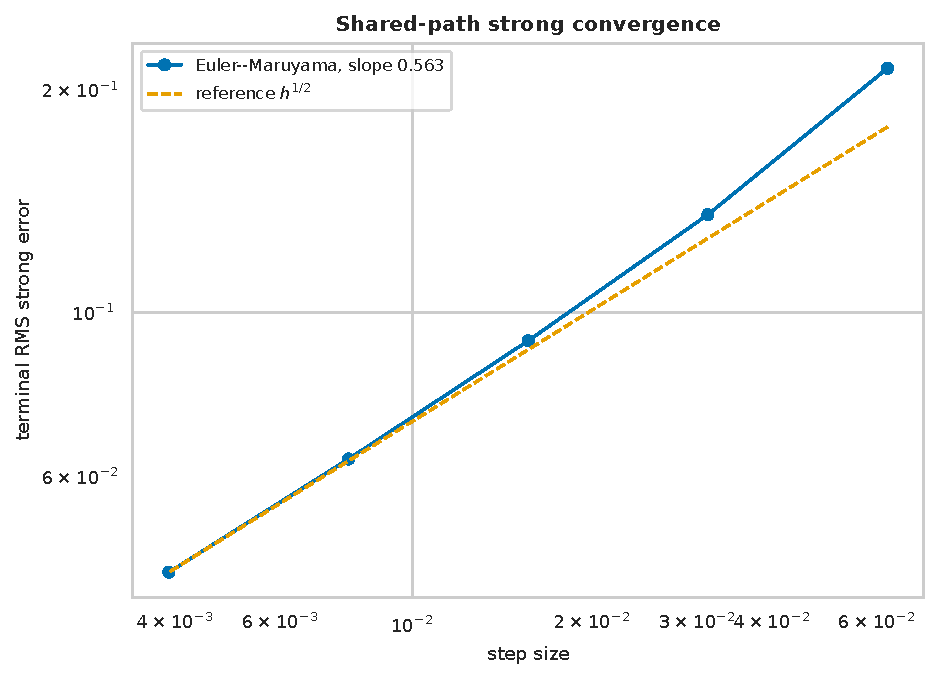
\includegraphics[width=0.76\linewidth,height=\textheight,keepaspectratio,alt={A log-log plot of Euler-\/-Maruyama terminal root-mean-square error follows the reference square-root step-size line on shared Brownian paths.}]{figures/vector/f16_strong_convergence.pdf}

}

\caption{\label{fig-strong-convergence}A log-log plot of Euler--Maruyama
terminal root-mean-square error follows the reference square-root
step-size line on shared Brownian paths.}

\end{figure}%

Figure~\ref{fig-strong-convergence} shows the expected order-\(1/2\)
trend. The exact transition Eq.~\ref{eq-exact-step} remains preferable
for this constant-coefficient model; Euler--Maruyama is included as a
numerical consistency check and a baseline for extensions without a
closed form.

\subsection{Quadratic variation}\label{quadratic-variation-1}

\begin{longtable}[]{@{}lllr@{}}
\caption{Quadratic-variation diagnostics from
\protect\texttt{tables/quadratic\_variation.csv}.}\label{tbl-brackets}\tabularnewline
\toprule\noalign{}
Bracket & Realized terminal value & Integral target & Relative error \\
\midrule\noalign{}
\endfirsthead
\toprule\noalign{}
Bracket & Realized terminal value & Integral target & Relative error \\
\midrule\noalign{}
\endhead
\bottomrule\noalign{}
\endlastfoot
bilinear & \(-0.21668-1.42167i\) & \(-0.21402-1.42148i\) & 0.00186 \\
Hermitian & 1.77059 & 1.76728 & 0.00187 \\
\end{longtable}

\begin{figure}[tbp]

\centering{

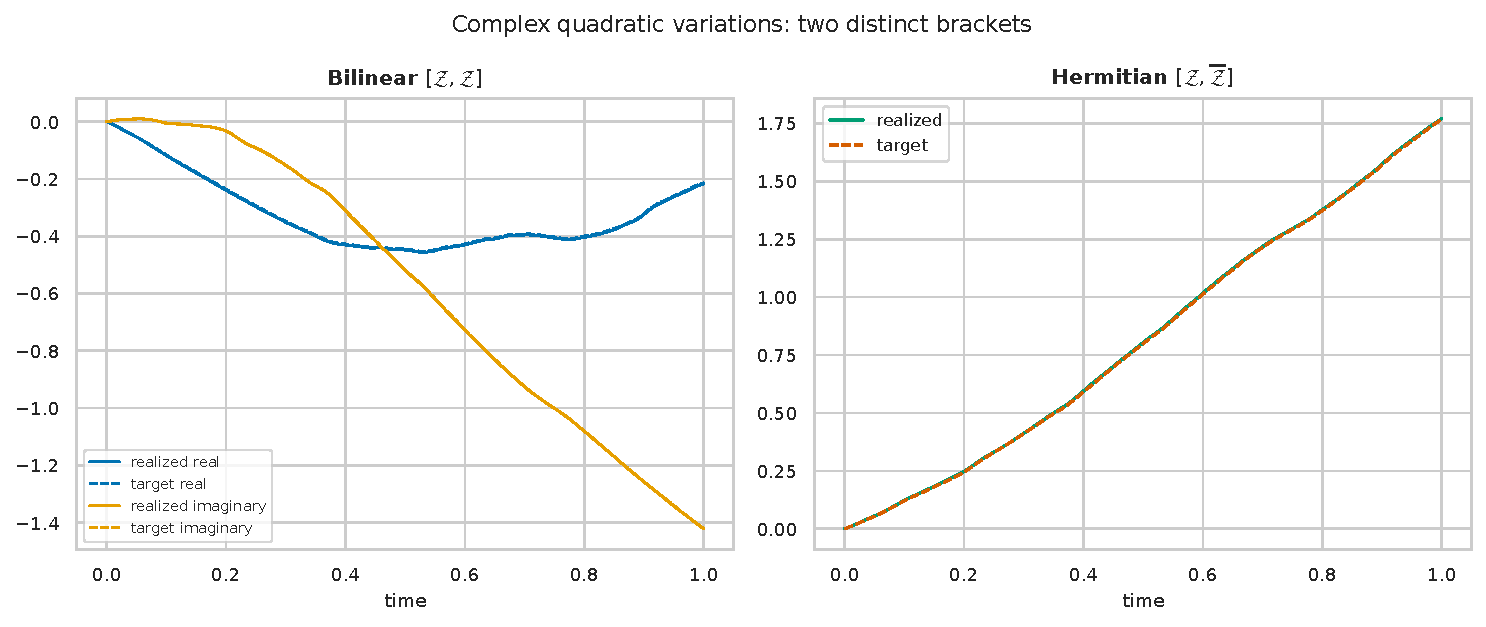
\includegraphics[width=0.95\linewidth,height=\textheight,keepaspectratio,alt={Cumulative realized bilinear and Hermitian complex quadratic variations track their analytic time-integral targets, with the bilinear bracket split into real and imaginary parts.}]{figures/vector/f17_complex_quadratic_variation.pdf}

}

\caption{\label{fig-complex-brackets}Cumulative realized bilinear and
Hermitian complex quadratic variations track their analytic
time-integral targets, with the bilinear bracket split into real and
imaginary parts.}

\end{figure}%

The simultaneous agreement in Figure~\ref{fig-complex-brackets} is a
useful guard against accidentally replacing \(B^2\) with \(|B|^2\).

\section{Discussion}\label{sec-discussion}

The construction achieves the requested elimination of an external
\(x\)-\(y\) state definition. The complete process is specified by one
term, \(\kappa t+BW_t\), inside one complex exponential. The real part
of that term is the log GBM; the imaginary part is the phase lift. The
corresponding exact finite-step walk has the same architecture.

The rotational role of Euler's formula is genuine. Multiplication by
\(e^{i\Delta\theta}\) rotates each state, and the imaginary Brownian
coefficient makes \(\Delta\theta\) random. What does \emph{not} follow
is an algebraic identification of \(i^2=-1\) with Brownian quadratic
variation. Instead, the square of the complex diffusion coefficient
enters because Itô's formula contains a quadratic-variation term. This
disciplined separation preserves both the geometric intuition and the
stochastic calculus.

The one-driver model produces strong scale--rotation dependence. A
positive Brownian shock changes log-radius by \(\sigma\,dW\) and phase
by \(\beta\,dW\) simultaneously. This may be a desired modeling feature.
If independent scale and rotation shocks are required,
Eq.~\ref{eq-two-driver-process} is the correct extension.

The ordinary exponential, stochastic exponential, exact random walk, and
Itô SDE are not competing formulas. They are equivalent views connected
by the half-bracket correction:

\begin{figure}[tbp]

\centering{

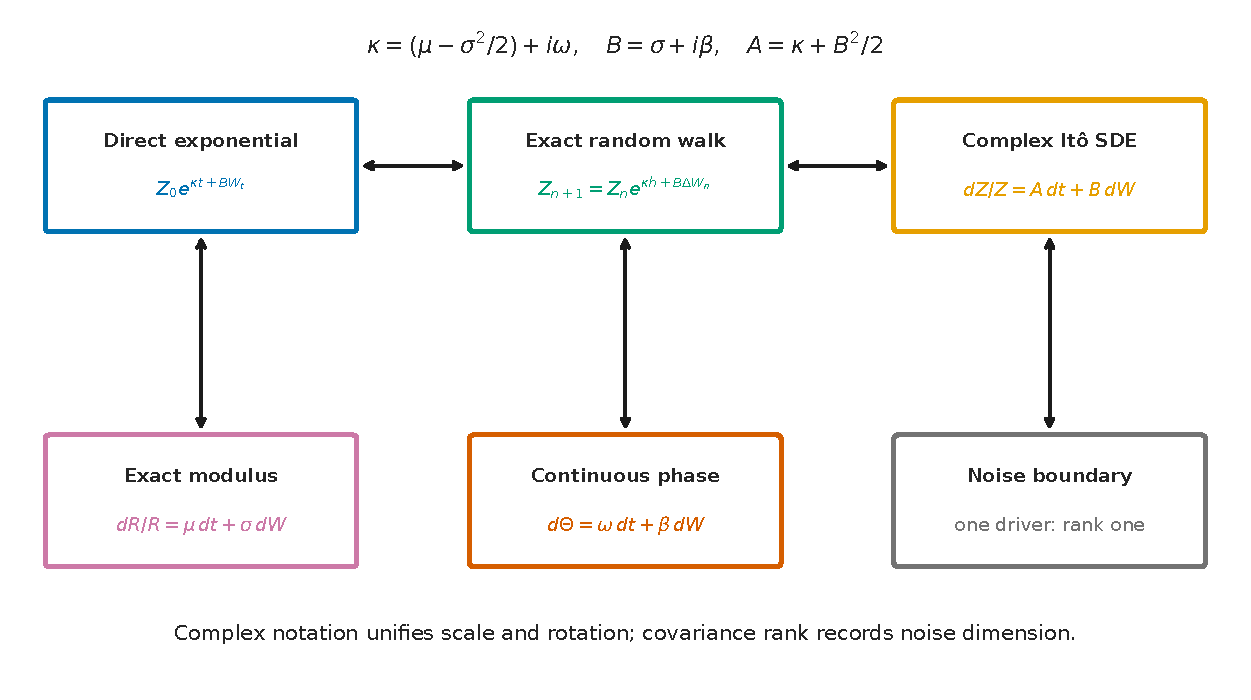
\includegraphics[width=1\linewidth,height=\textheight,keepaspectratio,alt={A taxonomy links the direct exponential, exact random walk, complex Itô SDE, exact GBM modulus, continuous phase, and rank-one noise boundary.}]{figures/vector/f18_representation_taxonomy.pdf}

}

\caption{\label{fig-taxonomy}A taxonomy links the direct exponential,
exact random walk, complex Itô SDE, exact GBM modulus, continuous phase,
and rank-one noise boundary.}

\end{figure}%

Figure~\ref{fig-taxonomy} is the compact answer to the session's design
goal.

\section{Limitations}\label{sec-limitations}

\begin{enumerate}
\def\labelenumi{\arabic{enumi}.}
\tightlist
\item
  \textbf{Established family.} The process belongs to the known complex
  scalar linear SDE/complex GBM family. The paper contributes a
  parameterization and synthesis, not a new existence theorem.
\item
  \textbf{One noise dimension.} A complex coefficient does not create an
  independent Brownian coordinate. Both log-radius and phase noise lie
  in a rank-one covariance direction.
\item
  \textbf{Singular fixed-time support.} For one driver, the joint
  log-polar law is singular and the complex fixed-time support is
  one-dimensional.
\item
  \textbf{Phase conventions.} The continuous phase requires a chosen
  initial lift. The principal argument remains discontinuous at its
  branch cut.
\item
  \textbf{No zeros.} The exponential construction stays in
  \(\mathbb C\setminus\{0\}\). It does not model paths that hit the
  origin.
\item
  \textbf{Constant coefficients.} Exact transition and closed-form
  moments rely on constant coefficients. State-dependent or noncommuting
  matrix extensions require additional analysis.
\item
  \textbf{No planar Brownian claim.} Classical planar Brownian motion
  and its winding laws (Spitzer 1958; Pitman and Yor 1986) are not laws
  of this one-driver process.
\item
  \textbf{No financial assertion.} Although GBM terminology is standard
  in mathematical finance, this paper makes no pricing, calibration, or
  no-arbitrage claim.
\end{enumerate}

\section{Conclusion}\label{sec-conclusion}

The design objective admits one concise native complex form:

\[
\boxed{
\mathcal Z_t
=
\mathcal Z_0
\exp\!\left(
\left[\left(\mu-\frac12\sigma^2\right)+i\omega\right]t
+(\sigma+i\beta)W_t
\right).
}
\]

Its exact random-walk transition is

\[
\boxed{
\mathcal Z_{n+1}
=
\mathcal Z_n
\exp\!\left(
\left[\left(\mu-\frac12\sigma^2\right)+i\omega\right]h
+(\sigma+i\beta)\Delta W_n
\right).
}
\]

Its equivalent complex Itô SDE is

\[
\boxed{
\frac{d\mathcal Z_t}{\mathcal Z_t}
=
\left[
\mu-\frac12\beta^2+i(\omega+\sigma\beta)
\right]dt
+(\sigma+i\beta)dW_t.
}
\]

The modulus is exactly the desired real GBM, and the imaginary exponent
provides deterministic and stochastic rotation. The cross drift and
rank-one covariance are not incidental: they precisely record the use of
one shared real Brownian driver. In this way, complex notation supplies
a unified scale--rotation language while covariance rank keeps the
stochastic dimension honest.

\section{Appendix A: Expanded Itô algebra}\label{sec-appendix-ito}

Write

\[
\Lambda_t=U_t+iV_t,
\]

where

\[
dU_t
=
\left(\mu-\frac12\sigma^2\right)dt+\sigma\,dW_t,
\]

\[
dV_t=\omega\,dt+\beta\,dW_t.
\]

In quadratic-covariation notation, the two real processes have Itô
products

\[
(dU_t)^2=\sigma^2dt,\qquad
(dV_t)^2=\beta^2dt,\qquad
dU_t\,dV_t=\sigma\beta\,dt.
\]

Since

\[
\mathcal Z_t=\mathcal Z_0e^{U_t}(\cos V_t+i\sin V_t),
\]

one may apply the two-dimensional real Itô formula. More compactly,

\[
(d\Lambda_t)^2
=(dU_t+i\,dV_t)^2
=
(dU_t)^2-(dV_t)^2+2i\,dU_t\,dV_t,
\]

so

\[
(d\Lambda_t)^2
=
(\sigma^2-\beta^2+2i\sigma\beta)dt
=B^2dt.
\]

Then

\[
\frac{d\mathcal Z_t}{\mathcal Z_t}
=d\Lambda_t+\frac12(d\Lambda_t)^2,
\]

which expands to Eq.~\ref{eq-final-sde}. This calculation makes clear
that the imaginary cross drift arises from \(dU_t\,dV_t\), the shared
Brownian covariation.

\section{Appendix B: Moment derivations}\label{sec-appendix-moments}

For any complex \(c\),

\[
\mathbb E[e^{cW_t}]=e^{c^2t/2},
\]

by analytic continuation of the Gaussian moment-generating function. For
the radial moment, substitute

\[
R_t^p
=R_0^p
e^{p(\mu-\sigma^2/2)t+p\sigma W_t}
\]

and use \(c=p\sigma\). This yields Eq.~\ref{eq-radial-moment}.

For the complex moment,

\[
\mathcal Z_t^n
=
\mathcal Z_0^n e^{n\kappa t+nBW_t},
\]

and \(c=nB\) yields Eq.~\ref{eq-complex-moment}.

Finally,

\[
R_t^p e^{iq(\Theta_t-\Theta_0)}
=
R_0^p
\exp\!\left[
p\left(\mu-\frac12\sigma^2\right)t
+iq\omega t
+\left(p\sigma+iq\beta\right)W_t
\right],
\]

which gives Eq.~\ref{eq-mixed-moment}.

\section{Appendix C: Reproducibility
manifest}\label{sec-appendix-reproducibility}

The canonical source is \texttt{index.qmd}. The discovery record is
\texttt{notebooks/phase4\_discovery.ipynb}, generated by
\texttt{notebooks/build\_phase4\_discovery.py}. The builder writes:

\begin{itemize}
\tightlist
\item
  18 vector figures under \texttt{figures/vector/};
\item
  18 raster companions under \texttt{figures/raster/};
\item
  coefficient, exactness, transition, covariance, moment, Phase 3,
  convergence, bracket, and software evidence under \texttt{tables/};
  and
\item
  figure and table manifests with stable relative paths.
\end{itemize}

Two clean notebook executions completed with sequential code-cell counts
1--9, no error outputs, identical code sources, identical deterministic
stream text, and the terminal marker
\texttt{ALL\_PHASE4\_ASSERTIONS\_PASSED}. The generated table hashes are
recorded in the project reproducibility guide.

The paper uses simulations to check implementation and illustrate
geometry. All the central identities---modulus, phase, Itô drift, exact
transition, moments, brackets, covariance rank, Phase 3 restrictions,
and two-driver drift---are analytical.

\protect\phantomsection\label{refs}
\begin{CSLReferences}{1}{1}
\bibitem[\citeproctext]{ref-abdulle2013}
Abdulle, Assyr, Gilles Vilmart, and Konstantinos C. Zygalakis. 2013.
{``Mean-Square a-Stable Diagonally Drift-Implicit Integrators of Weak
Second Order for Stiff {It{ô}} Stochastic Differential Equations.''}
\emph{BIT Numerical Mathematics} 53 (4): 827--40.
\url{https://doi.org/10.1007/s10543-013-0430-8}.

\bibitem[\citeproctext]{ref-buckwar2006}
Buckwar, Evelyn, Rózsa Horváth-Bokor, and Renate Winkler. 2006.
{``Asymptotic Mean-Square Stability of Two-Step Methods for Stochastic
Ordinary Differential Equations.''} \emph{BIT Numerical Mathematics} 46
(2): 261--82. \url{https://doi.org/10.1007/s10543-006-0060-5}.

\bibitem[\citeproctext]{ref-cernyruf2022}
Černý, Aleš, and Johannes Ruf. 2022. {``Simplified Stochastic Calculus
via Semimartingale Representations.''} \emph{Electronic Journal of
Probability} 27 (3): 1--32. \url{https://doi.org/10.1214/21-EJP729}.

\bibitem[\citeproctext]{ref-cernyruf2023}
Černý, Aleš, and Johannes Ruf. 2023. {``Simplified Calculus for
Semimartingales: Multiplicative Compensators and Changes of Measure.''}
\emph{Stochastic Processes and Their Applications} 161: 572--602.
\url{https://doi.org/10.1016/j.spa.2023.04.010}.

\bibitem[\citeproctext]{ref-doleansdade1970}
Doléans-Dade, Catherine. 1970. {``Quelques Applications de La Formule de
Changement de Variables Pour Les Semimartingales.''} \emph{Zeitschrift
f{ü}r Wahrscheinlichkeitstheorie Und Verwandte Gebiete} 16: 181--94.

\bibitem[\citeproctext]{ref-higham2001}
Higham, Desmond J. 2001. {``An Algorithmic Introduction to Numerical
Simulation of Stochastic Differential Equations.''} \emph{SIAM Review}
43 (3): 525--46. \url{https://doi.org/10.1137/S0036144500378302}.

\bibitem[\citeproctext]{ref-ito1951}
Itô, Kiyosi. 1951. {``On a Formula Concerning Stochastic
Differentials.''} \emph{Nagoya Mathematical Journal} 3: 55--65.
\url{https://doi.org/10.1017/S0027763000012216}.

\bibitem[\citeproctext]{ref-larssonruf2019}
Larsson, Martin, and Johannes Ruf. 2019. {``Stochastic Exponentials and
Logarithms on Stochastic Intervals---a Survey.''} \emph{Journal of
Mathematical Analysis and Applications} 476 (1): 2--12.
\url{https://doi.org/10.1016/j.jmaa.2018.11.040}.

\bibitem[\citeproctext]{ref-mora2015}
Mora, Carlos M., Juan C. Jimenez, and Hector Selva. 2015. {``A Stable
Numerical Scheme for Stochastic Differential Equations with
Multiplicative Noise.''} \emph{SIAM Journal on Numerical Analysis} 53
(4): 1613--41. \url{https://doi.org/10.1137/140984488}.

\bibitem[\citeproctext]{ref-mortersperes2010}
Mörters, Peter, and Yuval Peres. 2010. \emph{Brownian Motion}. Cambridge
Series in Statistical and Probabilistic Mathematics 30. Cambridge
University Press. \url{https://doi.org/10.1017/CBO9780511750489}.

\bibitem[\citeproctext]{ref-perret2010}
Perret, Christian. 2010. {``The Stability of Numerical Simulations of
Complex Stochastic Differential Equations.''} Doctoral Dissertation No.
18868. ETH Z{ü}rich. \url{https://doi.org/10.3929/ethz-a-006026507}.

\bibitem[\citeproctext]{ref-pitmanyor1986}
Pitman, Jim, and Marc Yor. 1986. {``Asymptotic Laws of Planar Brownian
Motion.''} \emph{The Annals of Probability} 14 (3): 733--79.
\url{https://doi.org/10.1214/aop/1176992436}.

\bibitem[\citeproctext]{ref-spitzer1958}
Spitzer, Frank. 1958. {``Some Theorems Concerning 2-Dimensional Brownian
Motion.''} \emph{Transactions of the American Mathematical Society} 87
(1): 187--97. \url{https://doi.org/10.1090/S0002-9947-1958-0104296-5}.

\end{CSLReferences}




\end{document}
